% !TeX root = RJwrapper.tex
\title{A Framework for Producing Small Area Estimates Based on Area-Level Models in R}


\author{by Sylvia Harmening, Ann-Kristin Kreutzmann, Sören Schmidt, Nicola Salvati, and Timo Schmid}

\maketitle

\abstract{%
The R package \href{https://CRAN.R-project.org/package=emdi}{emdi} facilitates the estimation of regionally disaggregated indicators using small area estimation methods and provides tools for model building, diagnostics, presenting, and exporting the results. The package version 1.1.7 includes unit-level small area models that rely on access to micro data. The area-level model by Fay and Herriot (1979) and various extensions have been added to the package since the release of version 2.0.0. These extensions include (a) area-level models with back-transformations, (b) spatial and robust extensions, (c) adjusted variance estimation methods, and (d) area-level models that account for measurement errors. Corresponding mean squared error estimators are implemented for assessing the uncertainty. User-friendly tools like a stepwise variable selection, model diagnostics, benchmarking options, high quality maps and results exportation options enable a complete analysis procedure. The functionality of the package is illustrated by examples based on synthetic data for Austrian districts.
}

\hypertarget{sec:intro}{%
\section{Introduction}\label{sec:intro}}

Small area estimation (SAE) enables better insight at smaller scales,
for which it has gained importance in both academic and applied
research. Among others, SAE is used for estimating socio-economic
measures like income, poverty and health or indicators for agriculture
(Datta, Fay, and Ghosh 1991; Tzavidis et al. 2012; Zhang et al. 2015; Pratesi 2016). Economic or
political decision-makers and official statistics practitioners
especially benefit from reliable estimation of disaggregated indicators
and thus SAE methods. Existing surveys were often not planned for
analysis at disaggregated levels and show only small sample sizes, which
leads to a low precision of the estimates. SAE methods can be employed
to avoid expensive and time-consuming enlargements of the sample size of
surveys. The idea is to combine data sources with model-based
approaches. Existing survey data will be enriched by auxiliary
information, e.g., from census or register data, to improve the accuracy
of the indicator estimation on an area- or domain- level. The terms area
and domain are used interchangeably and refer either to a geographic
area or to any subpopulation of a population of interest, like
socio-demographic groups. Among others, Pfeffermann (2013), Rao and Molina (2015),
Tzavidis et al. (2018) and Jiang and Rao (2020) give comprehensive overviews of SAE
methods.

The main goal of the package
\href{https://CRAN.R-project.org/package=emdi}{emdi} is the simplification of
estimating these regionally disaggregated indicators. The package
version 1.1.7 contains direct estimation based exclusively on survey
data and model-based estimation using the unit-level empirical best
predictor (EBP) method (Molina and Rao 2010). The EBP approach is powerful since
it enables the simultaneous estimation of various indicators. For this,
it relies on unit-level information, i.e.~information about each unit in
each domain. Though survey data often provides unit-level information,
access to census or register data at unit-level is less likely. Hence,
area-level models provide a valuable alternative, with the following
benefits: First, only area-level aggregates are needed to estimate the
regional indicators. Second, area-level models can consider the survey
design by integrating the sampling weights. Third, the computation is
faster compared to the computational intensive EBP approach.

Various R packages that employ different area-level models are available
on the Comprehensive R Archive Network (CRAN). The package
\href{https://CRAN.R-project.org/package=smallarea}{smallarea} (Nandy, 2015)
offers several variance estimation methods for the standard Fay-Herriot
(FH) model: maximum likelihood (ML), residual maximum likelihood (REML),
and both Prasad-Rao and Fay-Herriot method-of-moment. Estimation of
unknown sampling variances is also offered." The ability to estimate
unit- and area-level models under heteroscedasticity is implemented by
the \href{https://CRAN.R-project.org/package=JoSAE}{JoSAE} package
(Breidenbach 2018). Robust estimation of area-level models with spatial
and/or temporal structures in the random effects is supported by package
\href{https://CRAN.R-project.org/package=saeRobust}{saeRobust}
(Sebastian Warnholz 2022). The
\href{https://CRAN.R-project.org/package=mcmcsae}{mcmcsae} package
(Boonstra 2021) also takes spatial and temporal correlation of the
random effects into account, but fits unit- and area-level models via
Markov Chain Monte Carlo simulation. Estimation of univariate and
multivariate FH models is possible with package
\href{https://CRAN.R-project.org/package=msae}{msae} (Permatasari and Ubaidillah 2022). The
package \href{https://CRAN.R-project.org/package=hbsae}{hbsae}
(Boonstra 2022) allows for the fitting of unit- and area-level models by
frequentist or hierarchical Bayesian approaches. The possibility of
estimating FH models and some of its extensions in a Bayesian framework
is also given by the
\href{https://CRAN.R-project.org/package=BayesSAE}{BayesSAE} package
(Developer 2018). The
\href{https://CRAN.R-project.org/package=tipsae}{tipsae} package
(De Nicolò and Gardini 2022) provides estimation and mapping tools within a Bayesian
setting for proportions that are defined on the unit interval. The
\href{https://CRAN.R-project.org/package=mme}{mme} package (Lopez-Vizcaino, Lombardia, and Morales 2019)
implements Gaussian area-level multinomial mixed-effects models in the
SAE context. The \href{https://CRAN.R-project.org/package=saeME}{saeME}
package (Mubarak and Ubaidillah 2022) can fit an area-level model when the auxiliary
variables are measured with error. The
\href{https://CRAN.R-project.org/package=NSAE}{NSAE} package (Hukum Chandra et al. 2022)
can fit stationary and nonstationary FH models. One of the commonly used
packages is the \href{https://CRAN.R-project.org/package=sae}{sae} package
(Molina and Marhuenda 2015). It includes a wide range of area-level models (the
standard FH model with REML, ML and FH method-of-moment model fitting
and a spatial and a spatio-temporal extension of the FH model) and
unit-level models (the nested error linear regression model of
Battese, Harter, and Fuller (1988) and the EBP approach).
Table~\protect\hyperlink{tab:packages}{\[tab:packages\]} gives an overview of selected packages and the
implemented methodology.\\
Besides packages that include particular area-level models, the packages
\href{https://CRAN.R-project.org/package=saeMSPE}{saeMSPE} (Xiao et al. 2022) and
\href{https://CRAN.R-project.org/package=SAEval}{SAEval} (Fasulo 2022) offer
different analytical- and resampling-based MSE estimators and tools for
diagnostics and graphical evaluation of SAE models, respectively.

The latest version of package emdi 2.1.3 combines a wide range of SAE
models with several tools that enable a complete analysis, and therefore
adds to the space of useful packages, for the following reasons:

\begin{itemize}
\item
  None of the existing packages contains such a variety of different
  area-level models.
\item
  In addition to models that are already available in existing R
  packages, emdi includes: adjusted variance estimation methods and
  transformation options for the standard FH model. Adjusted variance
  estimation methods are of particular importance when working in a
  non-Bayesian framework. In a Bayesian context, the variance will
  always be estimated as strictly positive, so packages providing a
  Bayesian approach do not need adjusted variance estimation methods.
\item
  Package emdi offers user-friendly tools that go beyond model
  estimation: diagnostic tools with both summary and graphical
  results, benchmarking options, high-quality geographical
  visualization of results, and export of results to Excel and
  OpenDocument Spreadsheet formats.
\item
  Plus a stepwise variable selection algorithm for area-level models
  is included in emdi to allow the user to build a model based on
  information criteria.
\end{itemize}

Thus, since package version 2.0.0, version 1.1.7 has been extended by
various area-level models, but stays in line with the user-friendly
orientation of the existing version.

The structure of the paper can be described as follows. The section~
introduces the statistical methods implemented in the package. The
example data sets included in the package are presented in the section~.
The section~ provides an illustrative description of the functions using
the example data sets. The section ~ guides the reader from
model-building to diagnostics of a standard FH model and creating maps
of the results. The section ~ follows with short descriptions of how to
build the different extended area-level models. Finally, the section~
summarizes our contributions and gives an outlook.

@X @z @z @z @z @z @z @z @z @z \&\\

Area-level model \&

70 smallarea

\&

70 JoSAE

\&

70 sae

\&

70 saeRobust

\&

70 msae

\&

70 hbsae

\&

70 BayesSAE

\&

70 saeME

\&

70 emdi

\hfill\break

Standard variance estimation \& \(\surd\) \& \& \& \& \(\surd\) \& \(\surd\) \& \& \&
\(\surd\)\\

Adjusted variance estimation \& \& \& \& \& \& \& \& \& \(\surd\)\\

Unknown sampling variances \& \(\surd\) \& \& \& \& \& \& \& \&\\

Heteroscedasticity \& \& \(\surd\) \& \& \& \& \& \& \&\\

Spatial correlation \& \& \& \(\surd\) \& \& \& \& \& \& \(\surd\)\\

Spatio-temporal correlation \& \& \& \(\surd\) \& \& \& \& \& \&\\

Robust \& \& \& \& \(\surd\) \& \& \& \& \& \(\surd\)\\

Robust, spatial correlation \& \& \& \& \(\surd\) \& \& \& \& \& \(\surd\)\\

Robust, (spatio-)temporal correlation \& \& \& \& \(\surd\) \& \& \& \& \&\\

Multivariate \& \& \& \& \& \(\surd\) \& \& \& \&\\

Bayesian formulation \& \& \& \& \& \& \(\surd\) \& \(\surd\) \& \&\\

Measurement error \& \& \& \& \& \& \& \& \(\surd\) \& \(\surd\)\\

Transformation (log, arcsin) \& \& \& \& \& \& \& \& \& \(\surd\)\\

\hypertarget{sec:models}{%
\section{Statistical methodology}\label{sec:models}}

Area-level models for the estimation of indicators like means, totals or
shares have been added to the package since the release of version
2.0.0. These comprise the area-level model by Fay and Herriot (1979) and several
extensions of this standard model which account for issues that may come
up in real data applications. To measure the precision of those models,
MSE estimators have been integrated following the literature.

\hypertarget{subsec:stdfh}{%
\subsection{Standard Fay-Herriot model}\label{subsec:stdfh}}

Throughout the paper, a finite population \(U\) is assumed that consists
of \(N\) units that are subdivided into \(D\) domains or areas of specific
sizes \(N_1,...,N_D\). Then a random sample of size \(n\) can be drawn from
\(U\) and partitioned into \(D\) areas with \(n_1, ..., n_D\) observations per
domain.

The FH model links area-level direct estimators based on survey data to
covariates aggregated on an area level that may stem from administrative
data (e.g.~register or census) or alternative data sources (e.g.
satellite, social media or mobile phone data). The FH model is composed
of two levels. The first level is the sampling model
\[\hat{\theta}_{i}^{\text{Dir}}=\theta_{i} + e_{i}, \quad i=1,\ldots,D.\]
\(\hat{\theta}_{i}^{\text{Dir}}\) is an unbiased direct estimator for a
population indicator of interest \(\theta_{i}\), for instance, a mean or a
ratio. \(e_{i}\) represents independent and normally distributed sampling
errors with
\(e_{i} \stackrel{ind}{\sim} N\left(0,\sigma_{e_{i}}^2\right)\). Though
the model assumes known sampling variances, in practical applications
\(\sigma_{e_{i}}^2\) are usually unknown, and have to be estimated from
the unit-level sample data (Rivest and Vandal 2003; Wang and Fuller 2003; You and Chapman 2006). Package
emdi provides a non-parametric bootstrap for estimating the variances of
the direct estimator (Alfons and Templ 2013). To allow for complex survey designs,
sampling weights (\(w\)) can be considered in the direct estimation
(Horvitz and Thompson 1952). For example, an estimator for the population mean
\(\theta_{i}\) of a continuous variable of interest \(y\) for each area \(i\)
is estimated by \[\hat{\theta}_{i}^{\text{Dir}} =
\frac{\sum_{j=1}^{n_i} w_{ij} y_{ij}}{\sum_{j=1}^{n_i} w_{ij}},\] where
the index \(j\) indicates an individual with \(j = 1, ..., n_i\) in the
\(i\)-th area. The second FH level links the target indicator \(\theta_i\)
linearly to area-specific covariates \(\boldsymbol{x}_i\),
\[\theta_i = \boldsymbol{x}^{\top}_i \boldsymbol{\beta} +u_{i},\] where
\(\boldsymbol{\beta}\) is a vector of unknown fixed-effect parameters, and
\(u_i\) is an independent and identically normally distributed random
effect with
\(u_{i} \, \stackrel{iid}{\sim} N\left(0,\sigma_{u}^2\right)\).\\
The combination of the sampling and the linking model leads to a special
linear mixed model
\[\hat{\theta}_{i}^{\text{Dir}}=\boldsymbol{x}^{\top}_i \boldsymbol{\beta} +u_{i}
+ e_{i},
\quad i=1,\ldots,D.
\label{eq:Combination}\] The empirical best linear unbiased estimators
\(\boldsymbol{\hat{\beta}}\) are computed by weighted least square theory.
The empirical best linear unbiased predictor (EBLUP) of \(\theta_i\) is
obtained by substituting the variance parameter \(\sigma_u^2\) with an
estimate. The resulting estimator can then be written as
\[\begin{aligned}
\nonumber \hat{\theta}_i^{\text{FH}}&=
\boldsymbol{x}_i^{\top}\boldsymbol{\hat{\beta}} + \hat{u}_i \\
&=\hat{\gamma}_i\hat{\theta}_i^{\text{Dir}}+\left(1-\hat{\gamma}_i\right)
\boldsymbol{x}_i^{\top}\boldsymbol{\hat{\beta}}.
\label{eq:EBLUP}
\end{aligned}\] The EBLUP/FH estimator can be understood as a weighted
average of the direct estimator \(\hat{\theta}_i^{\text{Dir}}\) and a
regression-synthetic part
\(\boldsymbol{x}_i^{\top}\boldsymbol{\hat{\beta}}\). The estimated
shrinkage factor
\(\hat{\gamma}_i=\frac{\hat{\sigma}_u^2}{\hat{\sigma}_u^2+\sigma_{e_{i}}^2}\)
puts more weight on the direct estimator when the sampling variance is
small and vice versa. Areas for which no direct estimation results
exist, because the sample size is zero or the results may not be
published, are called out-of-sample domains. For those domains, the
prediction reduces to the regression-synthetic component
\(\hat{\theta}_{i,\text{out}}^{\text{FH}} = \boldsymbol{x}_i^{\top}\boldsymbol{\hat{\beta}}\) (Rao and Molina 2015).\\
\textbf{Estimation methods for} \(\boldsymbol{\sigma_u^2}\)\\
The variance of the random effects has to be estimated. Commonly used
approaches are the FH method-of-moment estimator (Fay and Herriot 1979), the ML, and
the REML estimators (Rao and Molina 2015). The likelihood methods are known to
perform more efficiently than the methods of moments (Rao and Molina 2015). The
commonly used methods can produce negative variance estimates that
should be strictly positive. In the estimation methods mentioned above,
negative variance estimates are set to zero (\(\hat{\sigma}_{u}^{2} = \max\left(\tilde{\sigma}_{u}^{2}, 0\right)\)) resulting in zero estimates
of the shrinkage factor \(\gamma_i\). Therefore, no weight is put on the
direct estimator, ignoring its possible reliability. This poses a
problem, especially when the number of areas is small. To avoid this
so-called over-shrinkage problem, Li and Lahiri (2010) and Yoshimori and Lahiri (2014) proposed
methods that adjust the respective likelihoods of the standard ML and
REML approaches by some factor:
\[L_{\text{adj}}\left(\sigma_u^{2}\right) = A \times L\left(\sigma_u^{2}\right),\]
where \(A\) denotes the adjustment factor and \(L(\sigma_u^{2})\) the given
likelihood function. The proposed adjustment factors are:

\begin{itemize}
\item
  by Li and Lahiri (2010): \(A = \sigma_u^{2}\),
\item
  by Yoshimori and Lahiri (2014): \(A = \left( \tan^{-1} \left(\sum\limits_{i=1}^{D}  \gamma_i \right)\right)^{1/D}\).
\end{itemize}

Simulation studies conducted by Yoshimori and Lahiri (2014) showed that the adjusted
Yoshimori-Lahiri methods are preferable when the variance of the random
effect is small relative to the sampling variance. Otherwise, the
adjusted Li-Lahiri methods are recommended. Package emdi offers six
different variance estimation methods: standard ML ( ml) and REML (
reml), and adjusted ML and REML following either Li and Lahiri (2010) ( amrl, ampl)
or Yoshimori and Lahiri (2014) ( amrl\_yl, ampl\_yl).

\hypertarget{subsec:extfh}{%
\subsection{Extended area-level models}\label{subsec:extfh}}

In real data applications, problems might occur that were not
theoretically expected. There may also be some violation of the
assumptions of the standard FH model, e.g., normality and independence
of the error terms. The following section outlines the extensions of the
standard FH model that are implemented in the package emdi to address
these issues.\\
\textbf{Transformations}\\
When working with right-skewed data like income, wealth or business
data, the assumptions of a linear relation between the response and the
explanatory variables and normality of both error terms (\(u_i\) and
\(e_i\)) of the FH model may be violated. Applying a log-transformation
could be a reasonable solution to meet these model assumptions
(Neves, Silva, and Correa 2013; A.-K. Kreutzmann et al. 2022). In the emdi package, the direct estimates
and their variances are transformed following Neves, Silva, and Correa (2013):
\[\begin{aligned}
\hat{\theta}_{i}^{\text{Dir*log}} &=
\log\left(\hat{\theta}_{i}^{\text{Dir}}\right), \\
\text{var}\left(\hat{\theta}_{i}^{\text{Dir*log}}\right) &=
\left(\hat{\theta}_{i}^{\text{Dir}}\right)^{-2}
\text{var}\left(\hat{\theta}_{i}^{\text{Dir}}\right),
\end{aligned}\] where the \(\text{*log}\) notation stands for the
logarithmic transformed scale. To obtain the FH estimator on the
transformed scale \(\hat{\theta}_i^{\text{FH*log}}\),
\(\hat{\theta}_{i}^{\text{Dir}}\) is substituted by
\(\hat{\theta}_{i}^{\text{Dir*log}}\) and
\(\text{var}(\hat{\theta}_{i}^{\text{Dir*log}})\) serves as estimate for
the sampling variances (\(\sigma_{e_{i}}^2\)) in
Equation~\protect\hyperlink{eq:EBLUP}{\[eq:EBLUP\]}. Since the logarithm is a nonlinear
transformation, the final FH estimates on the original scale require a
bias-corrected back-transformation (Slud and Maiti 2006; Sugawasa and Kubokawa 2017). The
emdi package provides two options:

\begin{enumerate}
\def\labelenumi{\arabic{enumi}.}
\item
  A \emph{crude} method ( bc\_crude) that takes the properties of the
  log-normal distribution into account:
  \[\hat{\theta}_i^{\text{FH, crude}} = \exp \left\{ \hat{\theta}_i^{\text{FH*log}} +
      0.5 \text{MSE}\left(\hat{\theta}_i^{\text{FH*log}}\right) \right\}.\]
\item
  A bias correction suggested by Slud and Maiti (2006) ( bc\_sm) that further
  regards the bias due to the random effects:
  \[\hat{\theta}^{\text{FH, Slud-Maiti}}_{i} = \exp\left\{ \hat{\theta}^{\text{FH*log}}_{i}
      + 0.5 \hat{\sigma}_{u}^{2} \left(1 - \hat{\gamma}_{i}^{\text{*log}}\right)\right\}.\]
\end{enumerate}

The FH estimator on the transformed scale is denoted by
\(\hat{\theta}_i^{\text{FH*log}}\) and, accordingly
\(\text{MSE}(\hat{\theta}_i^{\text{FH*log}})\) stands for a MSE estimator
on the transformed scale, e.g., the Prasad-Rao or Datta-Lahiri MSE (cf.
following subsection). The Slud-Maiti back-transformation is derived for
the ML variance estimation of the random effect and is implemented for
in-sample domains in emdi. In the presence of out-of-sample domains, the
\emph{crude} method can be applied, which allows to use also other variance
estimation methods.

Another transformation provided by the emdi package is the arcsin
transformation, which is widely used when the direct estimator of the FH
model is a ratio (Casas-Cordero, Encina, and Lahiri 2016; Schmid et al. 2017). The emdi package
automatically transforms the direct estimates and the sampling variances
as suggested by Jiang et al. (2001): \[\begin{aligned}
\hat{\theta}_{i}^{\text{Dir*arcsin}} &=
\sin^{-1}\left(\sqrt{ \left(\hat{\theta}_{i}^{\text{Dir}}\right)}\right), \\
\text{var}\left(\hat{\theta}_{i}^{\text{Dir*arcsin}}\right) &= 1 / \left(4 \tilde{n}_i\right),
\end{aligned}\] where the \(\text{*arcsin}\) denotes the arcsin
transformed scale, and \(\tilde{n}_i\) the effective sample size: the
sample size adjusted by the sampling design (Jiang et al. 2001). The FH model
is estimated using
Equation~\protect\hyperlink{eq:EBLUP}{\[eq:EBLUP\]} and, if necessary, the results are truncated to
the interval \([0, \pi / 2]\) to ensure final results between 0 and 1. To
obtain final estimates on the original scale, the final estimation
results must be subjected to a back-transformation. Two different
back-transformations are available in emdi:

\begin{enumerate}
\def\labelenumi{\arabic{enumi}.}
\tightlist
\item
  A \emph{naive} back-transformation ( naive):
  \[\hat{\theta}^{\text{FH, naive}}_{i} =
      \sin^2 \left(\hat{\theta}^{\text{FH*arcsin}}_{i}\right).\]
\end{enumerate}

\begin{enumerate}
\def\labelenumi{\arabic{enumi}.}
\tightlist
\item
  A back-transformation with bias-correction ( bc) following
  Sugawasa and Kubokawa (2017) and Hadam, Würz, and Kreutzmann (2020):
  \[\hat{\theta}^{\text{FH, bc}}_{i} = \int_{- \infty}^{\infty} \sin^2 \left(t\right)
      \frac{1}{2 \pi \frac{\hat{\sigma}^2_u \sigma^2_{e_i}}{\hat{\sigma}^2_u +
              \sigma^2_{e_i}}} \exp \left( - \frac{\left(t - \hat{\theta}^{\text{FH*arcsin}}_i
          \right)^2}{2 \frac{\hat{\sigma}^2_u \sigma^2_{e_i}}{\hat{\sigma}^2_u +
              \sigma^2_{e_i}}} \right) dt.\]
\end{enumerate}

\textbf{Spatial FH model}\\
The standard FH model assumes independence of the random effects.
However, when working with geographical areas, assuming correlated
random effects to incorporate a certain neighbouring structure can be
valuable. The emdi package contains the spatial FH model introduced by
Petrucci and Salvati (2006) that considers a simultaneously autoregressive process of
order one, SAR(1). Compared to the standard model, the estimation
differs mainly by discarding the assumptions of independent random
effects and estimating a spatial autoregressive coefficient (\(\rho\))
which takes values between \(-1\) and \(1\). Greater absolute values of
(\(\rho\)) indicate a stronger relationship with the neighboring areas.
The random effect \(u_i\) in
Equation~\protect\hyperlink{eq:Combination}{\[eq:Combination\]} is replaced by \[\begin{aligned}
\boldsymbol{u} = \rho_1 \boldsymbol{W} \boldsymbol{u} + \boldsymbol{\epsilon},
\text{   } \boldsymbol{\epsilon} \sim
N\left(\boldsymbol{0}_D,\sigma_{1}^2 \boldsymbol{I}_D\right),
\label{eq:u1}
\end{aligned}\] with \(\boldsymbol{W}\) being the \(D \times D\) row
standardized proximity matrix that describes the neighbourhood structure
of the areas, \(\boldsymbol{0}_D\) a vector of zeros and
\(\boldsymbol{I}_D\) the \(D \times D\) identity matrix. The random effects
\(\boldsymbol{u}\) of Equation~\protect\hyperlink{eq:u1}{\[eq:u1\]} follow a SAR(1). When normality of the random effects
is assumed, the model can be fitted by ML and REML. The application of
spatial FH models should be considered when no geographic auxiliary
variables are available to capture the spatial relation, or when
\(\rho_1\) is larger than 0.5 (Bertarelli et al. 2021). Even before estimating
the model, the emdi package enables testing for spatial correlation by
Moran's I and Geary's C statistics (Cliff and Ord 1981; Pratesi and Salvati 2008). While
Moran's I mimics a typical correlation coefficient whose values range
from \(-1\) and \(1\), Geary's C takes values between 0 and 2 (0: positive,
1: no, 2: negative spatial autocorrelation). The two statistics behave
inversely to each other.\\
\textbf{Robust area-level models}\\
In the case of influential outlying observations, the emdi package
allows for robust versions of the standard and the spatial FH model. The
theory is extensively studied in S. Warnholz (2016), wherein the robust
estimation procedure for linear mixed models suggested by Sinha and Rao (2009) was
extended to area-level models. The model fitting can be understood as a
robustified ML version that also contains an influence function with a
tuning constant k. 1.345 is recommended as an initial value for the
tuning constant (Sinha and Rao 2009). When non-symmetric outliers are expected
to influence the robust estimation, a bias correction should be
involved. This correction can be controlled by a multiplier constant (
mult\_constant). For further details, we also refer to R. Chambers et al. (2014) and
Schmid et al. (2016).\\
\textbf{Measurement error model}\\
The standard FH model is based on the assumption that the covariates are
measured without error (Fay and Herriot 1979). This characteristic is typically
assumed because census or register data are used as auxiliary
information. However, when the covariate information stems from larger
surveys or alternative data sources, this assumption can be violated.
The emdi package includes an implementation of the measurement error
(ME) model developed by Ybarra and Lohr (2008). To account for the ME in the
covariates \(\boldsymbol{x}_i\), they modified the shrinkage factor as
follows:
\[\gamma_i = \frac{\sigma_u^2 + \boldsymbol{\beta}^{\top} \boldsymbol{C}_i
    \boldsymbol{\beta}}{\sigma_u^2 + \boldsymbol{\beta}^{\top} \boldsymbol{C}_i
    \boldsymbol{\beta} + \sigma_{e_i}^2},\] where the \(\boldsymbol{C}_i\)
stands for the variance-covariance matrix of the covariates, which is a
required prerequisite for the model. The modified shrinkage factor pulls
more weight on the direct estimator when the variances of the covariates
are large. A modified weighted least squares method and a moment
estimator were used to estimate \(\boldsymbol{\beta}\)s and the
\(\sigma_u^2\), respectively. Additional details are available in
Ybarra and Lohr (2008).

\hypertarget{subsec:mseest}{%
\subsection{Mean squared error estimation}\label{subsec:mseest}}

To evaluate the accuracy of the EBLUP estimates, the MSE is the most
common measure used in SAE (Rao and Molina 2015). The emdi package offers a variety
of MSE estimators stemming from both analytical determination and
resampling strategies, like the bootstrap and jackknife methods.
Table~\protect\hyperlink{tab:overviewmse}{\[tab:overviewmse\]} gives an overview of the included MSE
approaches. For each area-level model presented in the previous
sections, the provided MSE types are shown. The quoted references detail
extensive formulas and derivations. As an additional measure of
variability of the direct and FH estimates, within various functions and
methods of the emdi package, the coefficient of variation (CV) is
provided:
\(CV = \sqrt{\widehat{\text{MSE}}(\hat{\theta}_{i})}/\hat{\theta}_{i}\),
where \(\hat{\theta}_{i}\) either stands for
\(\hat{\theta}_{i}^{\text{Dir}}\) or \(\hat{\theta}_{i}^{\text{FH}}\).

BXX Model \& Type of MSE \& Reference\\
\emph{Standard FH (depending on variance estimation of \(\sigma^2_{u}\))}\\
ml/ ampl\_yl \& Analytical \& Datta and Lahiri (2000)\\
reml/ amrl\_yl \& Analytical \& Prasad and Rao (1990)\\
ampl/ amrl \& Analytical \& Li and Lahiri (2010)\\
ml/ reml (out-of-sample) \& Analytical \& Rao and Molina (2015)\\
\emph{Transformations}\\
log (depending on back-transformation)\\
bc\_crude \& Analytical \& Rao and Molina (2015)\\
bc\_sm \& Analytical \& Slud and Maiti (2006)\\
arcsin (depending on back-transformation)\\
naive \& Jackknife \& Jiang et al. (2001)\\
\& Weighted Jackknife \& Jiang et al. (2001);\\
\& \& Chen and Lahiri (2002)\\
\& Parametric bootstrap \&

Hadam, Würz, and Kreutzmann (2020) bc \& Parametric bootstrap \& Hadam, Würz, and Kreutzmann (2020)\\
\emph{Spatial FH (depending on variance estimation)}\\
ml/ reml \& Analytical \& Singh, Shukla, and Kundu (2005)\\
ml/ reml \&

Parametric bootstrap \& Molina, Salvati, and Pratesi (2009)\\
reml \&

Nonparametric bootstrap \& Molina, Salvati, and Pratesi (2009)\\
\emph{Robust FH}\\
\& Pseudolinear \& S. Warnholz (2016)\\
\& Parametric bootstrap \& S. Warnholz (2016)\\
\emph{FH with ME}\\
\& Jackknife \& Jiang, Lahiri, and Wan (2002)\\

\hypertarget{sec:data}{%
\section{Data sets}\label{sec:data}}

The emdi package version 1.1.7 contains a sample
`{eusilcA\_smp}' and a population data set
`{eusilcA\_pop}' at a household level.

\hypertarget{tab:variables}{}
\begin{longtable}[]{@{}ll@{}}
\caption{Variables of the aggregated data sets. The Domain variables are
factors, the rest of the variables are numeric. Except for the
variables Domain and ratio\_n, the observations of all variables of the
population data set consist of the mean values per district.}\tabularnewline
\toprule\noalign{}
Variable & Meaning \\
\midrule\noalign{}
\endfirsthead
\toprule\noalign{}
Variable & Meaning \\
\midrule\noalign{}
\endhead
\bottomrule\noalign{}
\endlastfoot
\emph{Sample data set} & \\
Domain & Austrian districts \\
Mean & Mean of the equivalized household income \\
MTMED & Share of households who earn more than the national median income \\
Cash & Mean employee cash or near cash income \\
Var\_Mean & Variance of equivalized household income \\
Var\_MTMED & Variance of share of households who earn more than the national median income \\
Var\_Cash & Variance of employee cash or near cash income \\
n & Effective sample sizes \\
\emph{Population data set} & \\
Domain & Austrian districts \\
eqsize & Equivalized household size according to the modified OECD scale \\
cash & Employee cash or near cash income \\
self\_empl & Cash benefits or losses from self-employment (net) \\
unempl\_ben & Unemployment benefits (net) \\
age\_ben & Old-age benefits (net) \\
surv\_ben & Survivor's benefits (net) \\
sick\_ben & Sickness benefits (net) \\
dis\_ben & Disability benefits (net) \\
rent & Income from rental of a property or land (net) \\
fam\_allow & Family/children related allowances (net) \\
house\_allow & Housing allowances (net) \\
cap\_inv & Interest, dividends, profit from capital investments in unincorporated business (net) \\
tax\_adj & Repayments/receipts for tax adjustment (net) \\
ratio\_n & Ratios of the population size per area and the total population size \\
\end{longtable}

The generation process for both data sets is extensively described in
A.-K. Kreutzmann et al. (2019). Our process is nearly equivalent, but we do not produce
out-of-sample domains for the area-level version of the data sets. The
Austrian European Union Statistics on Income and Living Conditions
(EU-SILC) synthetic 2006 data set ( eusilcP) sourced from the
\href{https://CRAN.R-project.org/package=simFrame}{simFrame} package
(Alfons, Templ, and Filzmoser 2010) serves as basis for our data sets. The lowest
regional level in the eusilcP data set consists of the nine Austrian
states. Based on certain population size and income criteria, households
were allocated to 94 Austrian districts resulting in the synthetic
population data set `{eusilcA\_pop}'. For the
`{eusilcA\_smp}' data set, a sample was drawn following a
stratified random sampling process using the districts as strata. To
show the usage of the FH model and its extensions, area-level data is
required. The area-level survey and population data sets,
`{eusilcA\_smpAgg}' and `{eusilcA\_popAgg}', are
obtained by aggregation on the district level with the help of the
direct function defined by the emdi package. The direct estimates in
`{eusilcA\_smpAgg}' are the weighted mean equivalized
household income Mean, the ratio of households that earn more than the
national median income ( MTMED) and their variances. These are based on
the equivalized household income eqIncome in
`{eusilcA\_smp}', defined as the total income of a household
divided by the size of the household, with household size equalized by
the modified equivalence scale of the Organisation for Economic
Co-operation and Development (OECD) (Hagenaars, Vos, and Zaidi 1994). Additionally, the
mean of the variable cash, its variance and the sample sizes are
included in `{eusilcA\_smpAgg}', being required by the model
extensions. The population data set `{eusilcA\_popAgg}'
contains a variety of variables that describe different income sources
of households, and a variable ratio\_n that describes the ratios of the
population sizes per area and the total population size. The variable
Domain exists in both data sets and identifies the different districts.
Both data sets have an observation for each of the 94 Austrian
districts, with the sample data set `{eusilcA\_smpAgg}'
containing eight variables and the population data set
`{eusilcA\_popAgg}' containing fifteen.
Table~\protect\hyperlink{tab:variables}{1} provides an overview of all included
variables of the sample and population data sets. For the creation of
the proximity matrix used in the spatial FH model and the usage of the
map\_plot function, a shape file is needed. A shape file
`{shape\_austria\_dis}' ( .rda format,
"SpatialPolygonsDataFrame") for the 94 districts of Austria is
provided. This file was sourced from the SynerGIS website
(Bundesamt für Eich- und Vermessungswesen 2017). The data set `{eusilcA\_prox}', an example
proximity matrix, has also been added to the emdi package. The creation
of `{eusilcA\_prox}' is described in the following section.

\hypertarget{sec:functionality}{%
\section{Functionality and case studies}\label{sec:functionality}}

While the theoretical background of the implemented area-level models
has been introduced in the section~, the focus of this section lies on
the functionality and the workflow of their usage in R. All of the
contained area-level models can be applied by one function: fh.
Table~\protect\hyperlink{tab:inputfh}{\[tab:inputfh\]} gives an overview of the 20 input arguments of
function fh, together with a short description and any default settings.

B X n Argument \& Description \& Default\\
fixed \&

Formula of fixed-effects part of linear mixed model \&\\
vardir \&

Domain-specific sampling variances of the direct estimates\&\\
combined\_data \& Combined sample and census data set \&\\
domains \&

Domain indentifier for combined\_data \& NULL\\
method \& Model fitting method \& reml\\
interval \&

Lower and upper limit for the variance estimation \& NULL\\
k \& Tuning constant for robust estimation \& 1.345\\
mult\_constant \&

Bias correction multiplier constant for robust estimation \& 1\\
transformation \& Type of transformation \& no\\
backtransformation \& Type of back-transformation \& NULL\\
eff\_smpsize \& Effective sample sizes for the arcsin transformation \&
NULL\\
correlation \& Correlation of random effects \& no\\
corMatrix \& Proximity matrix for the spatial model \& NULL\\
Ci \&

Array of the variance-covariance matrix of the explanatory variables for
each area for the ME model \& NULL\\
tol \&

Tolerance value for the variance estimation \& 0.0001\\
maxit \&

Maximum number of iterations for the variance estimation \& 100\\
MSE \& MSE estimation \& FALSE\\
mse\_type \& Type of MSE estimator \& analytical\\
B \&

Numbers of bootstrap iterations for computation of a bootstrap MSE and
information criteria by Marhuenda, Morales, and Camen Pardo (2014) \& c(50,0)\\
seed \& Seed for random number generator \& 123\\

Not every argument needs a specification for every estimated model.
Depending on the area-level model, different arguments have to be
determined (see
Table~\protect\hyperlink{tab:inputarg}{\[tab:inputarg\]} in Appendix~A).
Figure~\protect\hyperlink{fig:flowstandard}{1} demonstrates the estimation possibilities
of a standard FH model (for the extended area-level models see
Figure~\protect\hyperlink{fig:flow}{16} in
Appendix A).

Overview of the standard FH model and adjusted variance
estimation methods.

In line with the direct and ebp functions of package version 1.1.7, the
S3 object system is used for function fh (J. Chambers and Hastie 1992). All three
return objects of class "emdi". The application of function direct
leads to a "direct" object, and of functions ebp and fh to objects of
classes "ebp" and "fh", respectively. Though all of the returned
objects contain ten components, not every component is available for
each estimation method. In these cases they are indicated as NULL (see
Table~\protect\hyperlink{tab:components}{\[tab:components\]}). Furthermore, the model component differs
for the two classes "ebp" and "fh". The components of objects of
class "fh" are provided in
Table~\protect\hyperlink{tab:modelcomp}{\[tab:modelcomp\]} in Appendix~B. Not all of the components are
available for every area-level model, e.g., the shrinkage factors per
domain are not provided for the spatial and robust model extensions, as
they do not have an intuitive interpretation in those cases. Due to the
consistent structure, all functions and methods of emdi version 1.1.7
can be applied to objects of class "fh". Additionally, new functions
and methods are available for the area-level models. Furthermore, a
variety of methods that are available in base R and used by other model
fitting R packages are included in the latest package version 2.1.3 for
the different "emdi" objects. Two examples of the new generic
functions used are coef and logLik.
Figure~\protect\hyperlink{fig:fct}{2}
demonstrates the steps of a full data analysis procedure and the
respective functions, from model building and diagnostics to presenting
the results. The section~ demonstrates the procedure shown in
Figure~\protect\hyperlink{fig:fct}{2} by
applying the standard FH model to the Austrian EU-SILC data described in
the section~. To demonstrate how the different extended area-level
models are fitted with function fh, the section~ follows.

@z @X @X @g @g @g \& Name \& Description \&\\
\& \& \& direct \& ebp \& fh\\
\& ind \& Point estimates per area \& \(\surd\) \& \(\surd\) \& \(\surd\)\\
2 \& MSE \&

Variance/MSE estimates per area \& \(\surd\) \& \(\surd\) \& \(\surd\)\\
3 \& transform\_param \&

Transformation and shift parameters \& \& \(\surd\) \&\\
4 \& model \& Fitted model \& \& \(\surd\) \& \(\surd\)\\
5 \& framework \& List for data description\& \(\surd\) \& \(\surd\) \& \(\surd\)\\
6 \& transformation \& Type of transformation \& \& \(\surd\) \& \(\surd\)\\
7 \& method \& Estimation method \& \& \(\surd\) \& \(\surd\)\\
8 \& fixed \& Formula of fixed effects \& \& \(\surd\) \& \(\surd\)\\
9 \& call \& Function call \& \(\surd\) \& \(\surd\) \& \(\surd\)\\
10 \& successful\_bootstraps \&

Number of successful bootstraps \& \(\surd\) \& \& \(\surd\)\\

\hypertarget{sec:functionalitystd}{%
\subsection{Estimation procedure for the standard Fay-Herriot model}\label{sec:functionalitystd}}

The aim of this example is to estimate the equivalized income for the 94
Austrian districts. The package and the example data sets are loaded as
follows:

\begin{example}
\textgreater{} library("emdi") \textgreater{} data("eusilcA\_popAgg") \textgreater{}
data("eusilcA\_smpAgg")
\end{example}

Estimation proce- dure for area-level models.

\textbf{Combine input data}\\
The function fh requires one data set (argument combined\_data) that
comprises the sample and population data. Thus, the data set must
contain all variables of the formula object fixed, the variances of the
direct estimates and, optionally, a domain identifier. For cases where
the sample and population data are only available separately, a merging
function combine\_data is provided. The necessary arguments are the two
data sets and characters specifying the domain indicator for the
respective data sets.

\begin{example}
\textgreater{} combined\_data \textless- combine\_data( + pop\_data = eusilcA\_popAgg,
pop\_domains = "Domain", + smp\_data = eusilcA\_smpAgg, smp\_domains =
"Domain")
\end{example}

\textbf{Identify spatial structures}\\
With the help of a proximity matrix, Moran's I and Geary's C test
statistics can be computed to identify spatial structures by the
spatialcor.tests command. For the creation of the proximity matrix, the
shapefile must be loaded. We load the Austrian shapefile that is
provided and merge it to the sample data set by using the respective
domain identifiers with the help of the merge method from the
\href{https://CRAN.R-project.org/package=sp}{sp} package (Pebesma and Bivand 2005).
Before merging, we sort the Austrian shapefile by the domains in the
sample data.

\begin{example}
\textgreater{} library("sp") \textgreater{} load\_shapeaustria() \textgreater{} shape\_austria\_dis \textless-
shape\_austria\_dis\[ + order(shape_austria_dis\$PB),\] \textgreater{} austria\_shape
\textless- merge(shape\_austria\_dis, + eusilcA\_smpAgg, by.x = "PB", by.y =
"Domain", + all.x = F)
\end{example}

Then the poly2nb and nb2mat functions of the
\href{https://CRAN.R-project.org/package=spdep}{spdep} package (Bivand and Wong 2018)
are used. While poly2nb generates a list of neighbours that share joint
boundaries, nb2mat computes a weights matrix. The style argument has to
be set to W, as a row standardized proximity matrix is required.

\begin{example}
\textgreater{} library("spdep") \textgreater{} rel \textless- poly2nb(austria\_shape, + row.names =
austria\_shape\(PB) > eusilcA_prox <- nb2mat(rel, style = "W", + zero.policy = TRUE) \end{example}  Thus, a row standardized proximity matrix is generated that initially had weights of one if an area shares a boundary with another area and zero if not. Function \texorpdfstring% {{\normalfont\ttfamily\hyphenchar\font=-1 spatialcor.tests}}% {spatialcor.tests} makes  use of the \texorpdfstring% {{\normalfont\ttfamily\hyphenchar\font=-1 moran.test}}% {moran.test} and \texorpdfstring% {{\normalfont\ttfamily\hyphenchar\font=-1 geary.test}}% {geary.test} functions with their respective  default settings, from the \texorpdfstring% {{\normalfont\fontseries{b}\selectfont spdep}}% {spdep} package. The input arguments are the created  matrix and the direct estimates. \begin{example} > spatialcor.tests(direct = combined_data
\)Mean, + corMatrix =
eusilcA\_prox)

Statistics Value p.value 1 Moran's I 0.2453677 5.607958e-05 2 Geary's C
0.6238681 2.473294e-03
\end{example}

Since the output indicates only a weak positive spatial autocorrelation,
the following estimation procedure does not consider the integration of
a correlation structure for the random effects.

\textbf{Perform model selection}

\hfill\break
Besides theoretical considerations on which auxiliary variables should
be part of the model, the decision for the best model should be based on
information criteria like the Akaike or Bayesian information criterion
(AIC, BIC). Many applications use selection techniques based on linear
regression (Casas-Cordero, Encina, and Lahiri 2016; Schmid et al. 2017). Instead, the emdi package provides
the AIC, BIC, Kullback information criterion (KIC) and their bootstrap
and bias corrected versions (AICc, AICb1, AICb2, KICc, KICb1, KICb2)
especially developed for FH models by Marhuenda, Morales, and Camen Pardo (2014). These criteria are
also included in the sae package, but the emdi package enables a
stepwise variable selection procedure based on the chosen information
criteria, comparable to the step function for lm models of package
stats. The most important input arguments are an object of class "fh"
and the direction of the stepwise search ( both, backward, forward). In
this example, the default setting backward and the KICb2 information
criterion is used. In the fixed argument of the fh function, the
variables employee cash ( cash), cash benefits from self-employment (
self\_empl) and unemployment benefits ( unempl\_ben) are included. For a
valid comparison of models based on information criteria, the model
fitting method must be ml. To activate the estimation of the information
criteria by Marhuenda, Morales, and Camen Pardo (2014), we set the number of bootstrap iterations to
50. The output shows the stepwise removal of variables until the lowest
KICb2 is reached, the function call and an overview of the estimated
coefficients of the final recommended model.

\begin{example}
\textgreater{} fh\_std \textless- fh(fixed = Mean ~ cash + self\_empl + unempl\_ben, vardir =
"Var\_Mean", + combined\_data = combined\_data, domains = "Domain",
method = "ml", B = c(0,50)) \textgreater{} step(fh\_std, criteria = "KICb2")

Start: KICb2 = 1709.42 Mean ~ cash + self\_empl + unempl\_ben

df KICb2 - unempl\_ben 1 1708.3 \textless none\textgreater{} 1709.4 - self\_empl 1 1763.0 -
cash 1 1808.6

Step: KICb2 = 1708.33 Mean ~ cash + self\_empl

df KICb2 \textless none\textgreater{} 1708.3 - self\_empl 1 1765.3 - cash 1 1816.1

Call: fh(fixed = Mean ~ cash + self\_empl, vardir = "Var\_Mean",
combined\_data = combined\_data, domains = "Domain", method = "ml", B
= c(0, 50))

Coefficients: coefficients std.error t.value p.value (Intercept)
3070.51231 635.94290 4.8283 1.377e-06 *** cash 1.05939 0.07049
15.0288 \textless{} 2.2e-16 *** self\_empl 1.74564 0.22017 7.9284 2.219e-15
*** --- Signif. codes: 0 `***' 0.001 `**' 0.01 `*' 0.05 `.' 0.1
' ' 1
\end{example}

KICb2 is minimised when the variable unempl\_ben is removed. Therefore,
the formula Mean \(\sim\) cash + self\_empl is used in the following.\\
\textbf{Estimate EBLUPs and MSEs}\\
The standard FH model is built. In addition to the fixed part, required
arguments are vardir and combined\_data. We specify the domains (if the
domains argument is set to NULL, the domains are numbered consecutively)
and activate the estimation of the MSE and of the information criteria
by Marhuenda, Morales, and Camen Pardo (2014).

\begin{example}
\textgreater{} fh\_std \textless- fh(fixed = Mean ~ cash + self\_empl, vardir = "Var\_Mean",
combined\_data = + combined\_data, domains = "Domain", method = "ml",
MSE = TRUE, B = c(0,50))
\end{example}

\textbf{Assess the estimated model}\\
In many publications using FH models, model diagnostics are discussed
only briefly, if at all. One reason for this might be the lack of an
existing implementation of desired diagnostic measures in R or other
statistical software. The summary method of emdi provides additional
information about the data and model components, in particular the
chosen estimation methods, the number of domains, the log-likelihood,
the information criteria by Marhuenda, Morales, and Camen Pardo (2014), the adjusted \(R^2\) of a
standard linear model and the adjusted \(R^2\) especially for FH models
proposed by Lahiri and Suntornchost (2015). Additionally, measures to validate model
assumptions about the standardized realized residuals and the random
effects are provided: skewness and kurtosis ( skewness and kurtosis of
package \href{https://CRAN.R-project.org/package=moments}{moments}, ) of the
standardized realized residuals and the random effects and the test
statistics with corresponding \(p\)~value of the Shapiro-Wilks-test for
normality of both error terms. As the introduced area-level models do
not assume a homoscedastic sampling distribution, the realized residuals
(\(\hat{e}_i\)) are standardized by
\(\hat{e}_i^{\text{std}} = \hat{e}_i / \sigma_{e_{i}}\) for the summary
and plot methods. The summary output differs slightly for the different
implemented area-level models. For example, log-likehoods and thus
information criteria are not available in theory for the robust and the
ME model.

\begin{example}
\textgreater{} summary(fh\_std)

Call: fh(fixed = Mean ~ cash + self\_empl, vardir = "Var\_Mean",
combined\_data = combined\_data, domains = "Domain", method = "ml",
MSE = TRUE, B = c(0, 50))

Out-of-sample domains: 0 In-sample domains: 94

Variance and MSE estimation: Variance estimation method: ml Estimated
variance component(s): 1371195 MSE method: datta-lahiri

Coefficients: coefficients std.error t.value p.value (Intercept)
3070.51231 635.94290 4.8283 1.377e-06 *** cash 1.05939 0.07049
15.0288 \textless{} 2.2e-16 *** self\_empl 1.74564 0.22017 7.9284 2.219e-15
*** --- Signif. codes: 0 `***' 0.001 `**' 0.01 `*' 0.05 `.' 0.1
' ' 1

Explanatory measures: loglike AIC AICc AICb1 AICb2 BIC KIC 1 -847.8303
1703.661 1703.91 1715.758 1703.461 1713.834 1707.661 KICc KICb1 KICb2
AdjR2 FH\_R2 1 1708.783 1720.632 1708.335 0.9212817 0.9482498

Residual diagnostics: Skewness Kurtosis Shapiro\_W Shapiro\_p
Standardized\_Residuals 0.3004662 3.971216 0.9840810 0.3119346
Random\_effects -0.4113238 3.086048 0.9839858 0.3072834

Transformation: No transformation
\end{example}

The output of the example shows that all domains have survey information
and the variance of \(\sigma_u^2\) amounts to 1371195. Further, all of the
included auxiliary variables are quite significant and their explanatory
power is large with an adjusted \(R^2\) (for FH models) of around 0.95.
The results of the Shapiro-Wilk-test indicate that normality is not
rejected for both errors. Graphical residual diagnostics are possible by
the plot method.

\begin{example}
\textgreater{} plot(fh\_std)
\end{example}

Figure~\protect\hyperlink{fig:plot}{6} shows
normal quantile-quantile (Q-Q) plots of the standardized realized
residuals and random effects
(Figure~\protect\hyperlink{fig:plota}{3}) as
well as plots of the kernel densities of the distribution of both error
terms and, for comparison, a standard normal distribution
(Figure~\protect\hyperlink{fig:plotb}{4}
and~\protect\hyperlink{fig:plotc}{5}). Like
in emdi version 1.1.7, the user is free to modify the interface of the
plots. The label and color arguments are easy to edit. Additionally, the
overall appearance of the plots are changeable by the gg\_theme argument,
as the plots are built with the
\href{https://CRAN.R-project.org/package=ggplot2}{ggplot2} package
(Wickham 2016). We refer to the package documentation for a detailed
description of how to customize the plot arguments.
Figure~\protect\hyperlink{fig:plot}{6}
supports the results of the normality tests provided in the summary
output, the distribution of the standardized random effects may be
slightly skewed (Figure~\protect\hyperlink{fig:plotc}{5}). If one is not be satisfied with the results,
applying a log-transformation could improve the distribution of the
error terms.

Output of plot(fh\_std): () normal quantile-quantile (Q-Q)
plots of the standardized realized residuals and random effects, () and
(): kernel densities of the distribution of the standardized realized
residuals and random effects (blue) in comparison to a standard normal
distribution (black).

\hfill\break
\textbf{Compare results with direct estimates}\\
The FH results should be consistent with the direct estimates for
domains with a small direct MSE and/or large sample sizes. Further, the
precision of the direct estimates should be improved by using auxiliary
information. The comparison of the direct and model-based (FH) estimates
can be done graphically by the generic function compare\_plot. For the fh
method the required input argument is an object of class "fh". When
the default settings of the command are used, the output consists of two
plots: a scatter plot proposed by Brown et al. (2001) and a line plot. Besides
the direct and FH estimates, the plot contains the fitted regression and
the identity line. These two lines should not differ too much.
Preferably, the model-based (FH) estimates should track the direct
estimates within the line plot especially for domains with a large
sample size or small MSE of the direct estimator. The points are ordered
by decreasing MSE of the direct estimates. In addition, the input
arguments MSE and CV can be set to TRUE leading to two extra plots,
respectively. The MSE/CV estimates of the direct and model-based (FH)
estimates are compared first via boxplots and second via ordered scatter
plots (ordered by increasing CV of the direct estimates). Like for the
plot command, a variety of customization options are offered, e.g., the
label options ( label), the format of the points ( shape) and the style
of the line ( line\_type).

\begin{example}
\textgreater{} compare\_plot(fh\_std, CV = TRUE, label = "no\_title")
\end{example}

Except one high value, the fitted regression and identity line of the
scatter plot (Figure~\protect\hyperlink{fig:comparea}{7}) are relatively close. Note that the high
value corresponds to the domain Eisenstadt (Stadt) with a very small
sample size of 10 and the highest MSE of the direct estimates, so the
direct estimator is very uncertain. Also the direct estimates are well
tracked by the model-based (FH) estimates within the line plot
(Figure~\protect\hyperlink{fig:compareb}{8}). The boxplot
(Figure~\protect\hyperlink{fig:comparee}{9}) and the ordered scatter plot
(Figure~\protect\hyperlink{fig:comparef}{10}) show that the precision of the direct
estimates could be improved by the usage of the FH model in terms of
CVs. Additionally, all of the CV values are less than 20\% which is a
common rule of the UK Office for National Statistics in order to
determine whether estimation results should be published
(Miltiadou 2020).

Output of compare\_plot(fh\_std): () and () scatter and line
plots of direct and model-based point estimates, () and () boxplot and
scatter plots of the CV estimates of the direct and model-based (FH)
estimates.

Further on, the function compare enables the user to compute a goodness
of fit diagnostic (Brown et al. 2001) and a correlation coefficient of the
direct estimates and the estimates of the regression-synthetic part of
the FH model (H. Chandra, Salvati, and Chambers 2015). Following Brown et al. (2001), the difference
between the model-based estimates and the direct estimates should not be
significant (null hypothesis). The Wald test statistic is specified as
\[W\left(\hat{\theta}_i^{\text{FH}}\right) = \sum_{i = 1}^{D} \frac{\left(\hat{\theta}_i^{\text{Dir}}-
    \hat{\theta}_i^{\text{FH}}\right)^2}{\widehat{\text{var}}\left(\hat{\theta}_i^{\text{Dir}}\right) + \widehat{\text{MSE}}\left(\hat{\theta}_i^{\text{FH}}\right)}\]
and is approximately \(\chi^2\)-distributed with \(D\) degrees of freedom.
When working with out-of-sample domains, those are not taken into
account, because the direct estimates and their variances are missing.
The input argument of function compare is an "fh" object.

\begin{example}
\textgreater{} compare(fh\_std)

Brown test

Null hypothesis: EBLUP estimates do not differ significantly from the
direct estimates

W.value Df p.value 46.97181 94 0.9999874

Correlation between synthetic part and direct estimator: 0.94
\end{example}

The results of the goodness of fit statistic and the correlation
coefficient confirm what the scatter and the line plot already
indicated. In the example the null hypothesis is not rejected and the
correlation coefficient indicates a strong positive correlation (0.94)
between the direct and model-based (FH) estimates.\\
\textbf{Benchmarking for consistent estimates}\\
The idea of benchmarking is that the aggregated FH estimates should sum
up to estimates of a higher regional level (\(\tau\)):
\[\sum_{i=1}^{D} \xi_{i} \hat{\theta}_{i}^{\text{FH, bench}} = \tau,\]
where \(\xi_{i}\) stands for the share of the population size of each area
in the total population size (\(N_{i}/N\)). In our example, the EBLUP
estimates could get aggregated on a national level and then compared to
or benchmarked with the Austrian mean equivalized income. The emdi
package contains a benchmark function that allows the user to select
three different options suggested by Datta et al. (2011). A general estimator of
the three options can be written as follows:
\[\hat{\theta}_{i}^{\text{FH, bench}} = \hat{\theta}_{i}^{\text{FH}} + \left( \sum_{i=1}^{D} \frac{\xi_{i}^2}{\phi_{i}} \right)^{-1} \left( \tau - \sum_{i=1}^{D} \xi_{i}\hat{\theta}_{i}^{\text{FH}}  \right) \frac{\xi_{i}}{\phi_{i}}.\]
Depending on the weight \(\phi_{i}\), the formula leads to different
benchmarking options. If \(\phi_{i}\) equals \(\xi_{i}\), all FH estimates
are adjusted by the same value ( raking). A ratio adjustment ( ratio) is
being conducted if \(\phi_{i} = \xi_{i}/\hat{\theta}_{i}^{\text{FH}}\).
For the last option ( MSE\_adj),
\(\phi_{i} = \xi_{i}/{\widehat{\text{MSE}}\left(\hat{\theta}_{i}^{\text{FH}}\right)}\).
While the first option is a relatively naive approach, the latter two
conduct larger adjustments for the areas with larger FH and MSE
estimates, respectively. Thus, for the benchmark function the following
arguments have to be specified: an object of class "fh", a benchmark
value, a vector containing the \(\xi_{i}\)s ( share) and the type of
benchmarking. The output is a data frame with an extra column FH\_Bench
for the benchmarked EBLUP values. If the optional argument overwrite is
set to TRUE, the benchmarked results are added to the "fh" object and
the MSE estimates of the non benchmarked FH estimates are set to NULL.
For the used example, the benchmark value is calculated by taking the
mean of the variable eqIncome of the `{eusilcA\_smp}' data
frame. The \(\xi_{i}\)s can be found in `{eusilcA\_popAgg}' as
ratio\_n.

\begin{example}
\textgreater{} fh\_bench \textless- benchmark(fh\_std, benchmark = 20140.09, share =
eusilcA\_popAgg\$ratio\_n,
+ type = ``ratio'')
\textgreater{} head(fh\_bench)

\begin{verbatim}
          Domain   Direct       FH FH_Bench Out
\end{verbatim}

1 Amstetten 14768.57 14242.04 14480.61 0
2 Baden 21995.72 21616.40 21978.49 0
3 Bludenz 12069.59 12680.38 12892.79 0
4 Braunau am Inn 10770.53 11925.82 12125.59 0
5 Bregenz 35731.20 32101.69 32639.43 0
6 Bruck-Mürzzuschlag 23027.37 22523.50 22900.79 0
\textbackslash end\{example\}
It is recognizable that for the first six Austrian districts the original estimates are slightly modified by the benchmarking.
\textbackslash{} \newline
\textbf{Extract and visualize the results} \textbackslash{}
To gain an overview of the point, MSE and CV results of the direct estimates compared to the model-based (FH) results the generic function \texorpdfstring%
{{\normalfont\ttfamily\hyphenchar\font=-1 estimators}}%
{estimators} \citep{emdi2019} can be used, but differences among areas or hotspots of special interest are usually easier to detect on maps. With function \texorpdfstring%
{{\normalfont\ttfamily\hyphenchar\font=-1 map\_plot}}%
{map\_plot}, the \texorpdfstring%
{{\normalfont\fontseries{b}\selectfont emdi}}%
{emdi} package offers a user-friendly way to produce maps since creating maps can often become a time consuming task. The input arguments mainly consist of an object of class \texorpdfstring%
{{\normalfont\ttfamily\hyphenchar\font=-1 "emdi"}}%
{"emdi"} and a spatial polygon of a shape file. The only issue that might come up is if domain identifiers in the data do not match to the respective identifiers of the shape file. In those cases, the input argument \texorpdfstring%
{{\normalfont\ttfamily\hyphenchar\font=-1 map\_tab}}%
{map\_tab} is required, which is a data frame that contains the matching of the domain indentifiers of the population and the shape file data sets. For detailed instructions, we refer to \citet{emdi2019} and to the help page of function \texorpdfstring%
{{\normalfont\ttfamily\hyphenchar\font=-1 map\_plot}}%
{map\_plot}.

For producing maps of the 94 Austrian districts, the Austrian shape file has to be loaded. In addition to the \texorpdfstring%
{{\normalfont\ttfamily\hyphenchar\font=-1 "emdi"}}%
{"emdi"} object, the \texorpdfstring%
{{\normalfont\ttfamily\hyphenchar\font=-1 "SpatialPolygonsDataFrame"}}%
{"SpatialPolygonsDataFrame"} object (\texorpdfstring%
{{\normalfont\ttfamily\hyphenchar\font=-1 map\_obj}}%
{map\_obj}) and a domain indicator (\texorpdfstring%
{{\normalfont\ttfamily\hyphenchar\font=-1 map\_dom\_id}}%
{map\_dom\_id}) have to be specified. The \texorpdfstring%
{{\normalfont\ttfamily\hyphenchar\font=-1 map\_tab}}%
{map\_tab} argument is not necessary since the identifiers match in our example. To allow for an easier comparison of the results, we adjust the scales of the maps using the \texorpdfstring%
{{\normalfont\ttfamily\hyphenchar\font=-1 scale\_points}}%
{scale\_points} argument.

\begin{example}
> load_shapeaustria()
> map_plot(object = fh_std, MSE = TRUE, map_obj = shape_austria_dis,
+   map_dom_id = "PB", scale_points = list(Direct = list(
+   ind = c(8000, 60000), MSE = c(200000, 10000000)), FH = list(
+   ind = c(8000, 60000), MSE = c(200000, 10000000))))
\end{example}
\begin{figure}[H]
    \begin{subfigure}[t]{0.49\textwidth}
        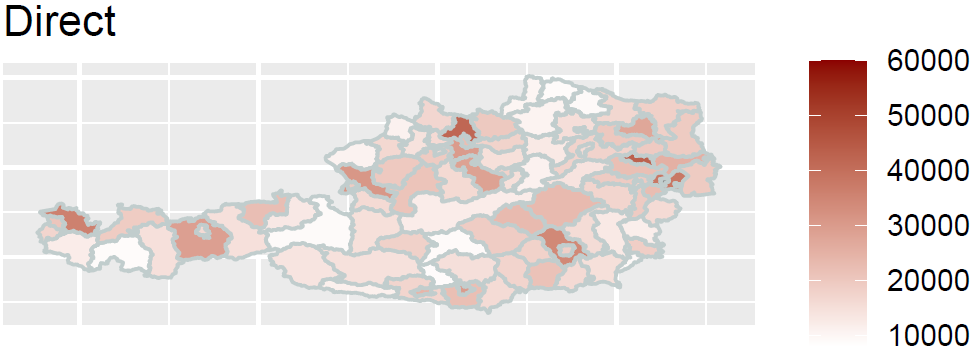
\includegraphics[width=\textwidth]{figures/map1.png}
        \caption{}
        \label{fig:mapa}
    \end{subfigure}\hfill%
    \begin{subfigure}[t]{0.49\textwidth}
        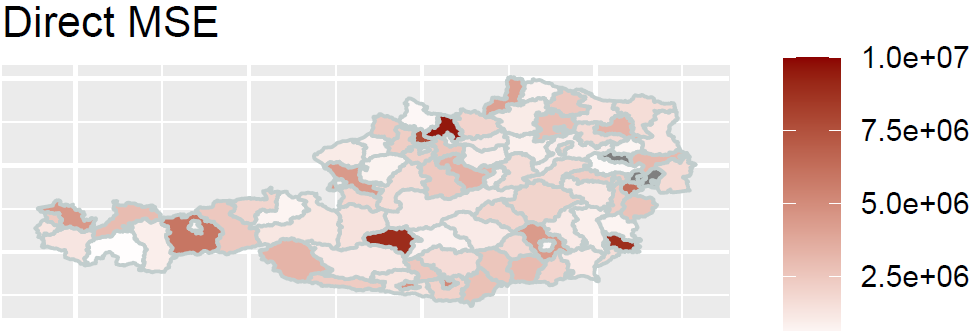
\includegraphics[width=\textwidth]{figures/map2.png}
        \caption{}
        \label{fig:mapb}
    \end{subfigure}\\[5pt]%
    %\centering
    \begin{subfigure}[t]{0.49\textwidth}
        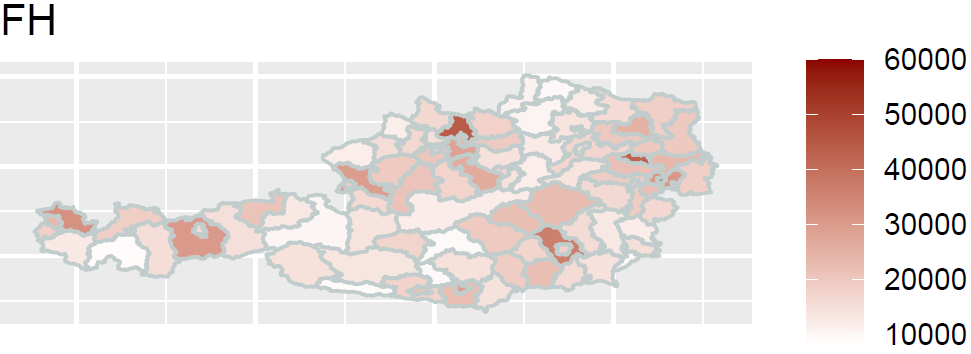
\includegraphics[width=\textwidth]{figures/map3.png}
        \caption{}
        \label{fig:mapc}
    \end{subfigure}\hfill%
    \begin{subfigure}[t]{0.49\textwidth}
        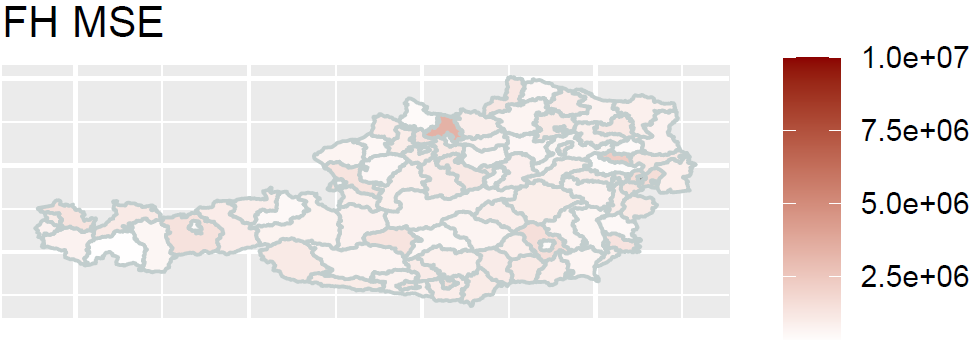
\includegraphics[width=\textwidth]{figures/map4.png}
        \caption{}
        \label{fig:mapd}
    \end{subfigure}%
    \caption{Output of \texorpdfstring%
{{\normalfont\ttfamily\hyphenchar\font=-1 map\_plot}}%
{map\_plot}: Maps of the direct and FH estimates ((\subref{fig:mapa}) and (\subref{fig:mapc})) with corresponding MSE estimates ((\subref{fig:mapb}) and (\subref{fig:mapd})).}
    \label{fig:mapplot}
\end{figure}

Figures\textasciitilde{}\ref{fig:mapa} and\textasciitilde{}\ref{fig:mapc} show the distribution of the estimated
(direct vs.~model-based) equivalized income across Austria. It is striking that
white and light red tones dominate the map, indicating relatively low mean
incomes of the districts. But in contrast, districts Eisenstadt
(Stadt), Urfahr-Umgebung and M"odling stand out having the largest incomes.
Urfahr-Umgebung is also eye-catching when having a look at the MSE estimates
(Figures\textasciitilde{}\ref{fig:mapb} and\textasciitilde{}\ref{fig:mapd}). The MSE of the direct and the FH
estimates are quite high. Probably a single wealthy household raised the mean
income and also the variance. Figure\textasciitilde{}\ref{fig:mapb} contains some districts with
MSEs larger than the customized scaling (gray areas). Without the scaling it would
have been hard to identify any differences in Figure\textasciitilde{}\ref{fig:mapd}.\\
\textbackslash{} \newline
\textbf{Export the results} \textbackslash{}
Some users might have an interest to store the results separately or to use them
for presentations. Excel and OpenDocument Spreadsheets provide many opportunities for that. In contrast
to some existing R packages, the \texorpdfstring%
{{\normalfont\fontseries{b}\selectfont emdi}}%
{emdi} functions \texorpdfstring%
{{\normalfont\ttfamily\hyphenchar\font=-1 write.excel}}%
{write.excel}/\texorpdfstring%
{{\normalfont\ttfamily\hyphenchar\font=-1 write.ods}}%
{write.ods}
do not only export the estimation results, but also the output of \texorpdfstring%
{{\normalfont\ttfamily\hyphenchar\font=-1 summary}}%
{summary}. Usage of the functions is comprehensively described in \citet{emdi2019}.

\subsection{Estimation of the extended area-level models} \label{sec:functionalityext}

\textbf{FH model with transformation} \textbackslash{}
If the indicator of interest needs a transformation, either log or arcsin, in addition to the function used in the previous subsection, the arguments \texorpdfstring%
{{\normalfont\ttfamily\hyphenchar\font=-1 transformation}}%
{transformation} and \texorpdfstring%
{{\normalfont\ttfamily\hyphenchar\font=-1 backtransformation}}%
{backtransformation} must be specified. If, for example, the share of households per area that earn more than the national median income (\texorpdfstring%
{{\normalfont\ttfamily\hyphenchar\font=-1 MTMED}}%
{MTMED}) is the indicator of interest, an arcsin transformation can be used. The bias-corrected back-transformation \texorpdfstring%
{{\normalfont\ttfamily\hyphenchar\font=-1 bc}}%
{bc} is chosen in the example. Two more arguments are needed when using an arcsin transformation: the name of the variable describing the effective sample sizes (\texorpdfstring%
{{\normalfont\ttfamily\hyphenchar\font=-1 eff\_smpsize}}%
{eff\_smpsize}) which needs to be contained in the \texorpdfstring%
{{\normalfont\ttfamily\hyphenchar\font=-1 combined\_data}}%
{combined\_data} frame. Because of having chosen the bias-corrected back-transformation, the only possible \texorpdfstring%
{{\normalfont\ttfamily\hyphenchar\font=-1 mse\_type}}%
{mse\_type} is \texorpdfstring%
{{\normalfont\ttfamily\hyphenchar\font=-1 boot}}%
{boot}, if the MSE estimation is activated.

\begin{example}
> fh_arcsin <- fh(fixed = MTMED ~ cash + age_ben + rent + house_allow,
+   vardir = "Var_MTMED", combined_data = combined_data, domains = "Domain",
+   transformation = "arcsin", backtransformation = "bc", eff_smpsize = "n",
+   MSE = TRUE, mse_type = "boot")
\end{example}

\textbf{Spatial FH model} \textbackslash{}
If the spatial correlation tests indicated a spatial correlation of the domains, a spatial FH model for incorporating the spatial structure in the model could be used. For that, the \texorpdfstring%
{{\normalfont\ttfamily\hyphenchar\font=-1 correlation}}%
{correlation} has to be set to \texorpdfstring%
{{\normalfont\ttfamily\hyphenchar\font=-1 spatial}}%
{spatial} and the example proximity matrix has to be given to the model within the \texorpdfstring%
{{\normalfont\ttfamily\hyphenchar\font=-1 corMatrix}}%
{corMatrix} argument. The possible variance estimation methods are \texorpdfstring%
{{\normalfont\ttfamily\hyphenchar\font=-1 ml}}%
{ml} and \texorpdfstring%
{{\normalfont\ttfamily\hyphenchar\font=-1 reml}}%
{reml}.

\begin{example}
> fh_spatial <- fh(fixed = Mean ~ cash + self_empl, vardir = "Var_Mean",
+   combined_data = combined_data, domains = "Domain", correlation = "spatial",
+   corMatrix = eusilcA_prox, MSE = TRUE)
\end{example}

\textbf{Robust FH model} \textbackslash{}
If extreme values could influence the estimation, the application of a robust model might be appropriate. Within the robust framework, package \texorpdfstring%
{{\normalfont\fontseries{b}\selectfont emdi}}%
{emdi} allows the user to choose between a standard and a spatial model (defaults to \texorpdfstring%
{{\normalfont\ttfamily\hyphenchar\font=-1 correlation}}%
{correlation} = \texorpdfstring%
{{\normalfont\ttfamily\hyphenchar\font=-1 "no"}}%
{"no"}). The estimation method must be \texorpdfstring%
{{\normalfont\ttfamily\hyphenchar\font=-1 reblup}}%
{reblup} or \texorpdfstring%
{{\normalfont\ttfamily\hyphenchar\font=-1 reblupbc}}%
{reblupbc} which includes a bias correction that can be modified by the argument \texorpdfstring%
{{\normalfont\ttfamily\hyphenchar\font=-1 mult\_constant}}%
{mult\_constant}. Further, the tuning constant \texorpdfstring%
{{\normalfont\ttfamily\hyphenchar\font=-1 k}}%
{k} defaults to 1.345 as proposed by \citet{Sinha2009} and \citet{Warnholz2016} and can be changed if desired. The functions of the package \texorpdfstring%
{{\normalfont\fontseries{b}\selectfont saeRobust}}%
{saeRobust} are utilized for the robust extensions. An exemplary call with pseudolinear MSE estimation looks like this:

\begin{example}
> fh_robust <- fh(fixed = Mean ~ cash + self_empl, vardir = "Var_Mean",
+   combined_data = combined_data, domains = "Domain", method = "reblup",
+   MSE = TRUE, mse_type = "pseudo")
\end{example}

\textbf{Measurement error model} \textbackslash{}
If other data sources than register data, e.g., data from larger surveys or big data sources are used as auxiliary information, the ME model should be applied. For the estimation of the ME model, the model fitting method must be set to \texorpdfstring%
{{\normalfont\ttfamily\hyphenchar\font=-1 me}}%
{me} and the only possible MSE estimation method is \texorpdfstring%
{{\normalfont\ttfamily\hyphenchar\font=-1 jackknife}}%
{jackknife}. The most complex input argument consists of the creation of the MSE array \texorpdfstring%
{{\normalfont\ttfamily\hyphenchar\font=-1 Ci}}%
{Ci}. The variability of the auxiliary variables that is taken into account by the ME model is expressed by the variance-covariance matrices per domain (\texorpdfstring%
{{\normalfont\ttfamily\hyphenchar\font=-1 Ci}}%
{Ci}). For example, for three covariates a, b and c the array should look like
\%
\begin{equation*}
\boldsymbol{C}_i = \left( \begin{array}{rrrr}
0 & 0 & 0 & 0 \\
0 & \text{var}_i(a) & \text{cov}_i(a,b) & \text{cov}_i(a,c) \\
0 & \text{cov}_i(a,b) & \text{var}_i(b) & \text{cov}_i(b,c) \\
0 & \text{cov}_i(a,c) & \text{cov}_i(b,c) & \text{var}_i(c) \\
\end{array}\right),
\text{   } i = 1,...,D.
\end{equation*}
\%
The first row and column contain zeros, because the intercept is considered. The variances and covariances can be computed by standard approaches like, for example, the Horvitz-Thompson estimator.

For the Austrian EUSILC data example, the equalized income can also be explained by a variable of the sample data set. The code below demonstrates how the MSE array \texorpdfstring%
{{\normalfont\ttfamily\hyphenchar\font=-1 Ci}}%
{Ci} is created for one covariate (variable \texorpdfstring%
{{\normalfont\ttfamily\hyphenchar\font=-1 Cash}}%
{Cash} and its variance \texorpdfstring%
{{\normalfont\ttfamily\hyphenchar\font=-1 Var\_Cash}}%
{Var\_Cash}) and how the final ME model is built.
\textbackslash begin\{example\}
\textgreater{} P \textless- 1
\textgreater{} M \textless- 94
\textgreater{} Ci\_array \textless- array(data = 0, dim = c(P + 1, P + 1, M))
\textgreater{} Ci\_array{[}2,2, {]} \textless- eusilcA\_smpAgg\$Var\_Cash

\textgreater{} fh\_yl \textless- fh(fixed = Mean ~ Cash, vardir = "Var\_Mean", +
combined\_data = eusilcA\_smpAgg, domains = "Domain", method = "me", +
Ci = Ci\_array, MSE = TRUE, mse\_type = "jackknife")
\end{example}

\hypertarget{sec:concl}{%
\section{Conclusion and outlook}\label{sec:concl}}

In this paper, we have presented how the emdi package version 1.1.7 has
been extended with various area-level models. Along with the well-known
FH model, adjusted variance estimation methods and transformation
options are offered to the user. In addition, spatial, robust, and ME
model extensions of the standard model allow the user to address various
issues that arise in practical data applications. All of these methods
can be estimated conveniently by using a single function that provides
EBLUP and the respective MSE estimates to measure their precision.
Especially in the section~, it is clear that the package does not only
contain tools for estimation of the different SAE models. Instead, it
additionally provides user-friendly tools to enable a whole data
analysis procedure: 1. starting with model building and estimation,
moving on to 2. model assessment and diagnostics, 3. presentation of the
results, and finishing with 4. exporting the results to Excel or
OpenDocument Spreadsheet.

For future package versions, it is planned to expand the options in the
field of area-level models. In some practical applications, the
incorporation of random effects is redundant. Therefore, an area-level
estimator that considers a preliminary testing for the random effects
following Molina, Rao, and Datta (2015) will be included. Since version 2.0.0 emdi
accounts for spatial structures of the random effects. Future
developments may also account for out-of-sample EBLUP and MSE estimation
for the spatial model proposed by Saei and Chambers (2005) and for temporal and
spatio-temporal extensions (Rao and Yu 1994; Marhuenda, Molina, and Morales 2013). For the existing
ME model, a bootstrap MSE estimation option may be added to the package
since the Jackknife MSE estimator may produce negative MSE estimates
(Marchetti et al. 2015). Furthermore, cross-validation options additional to
the model assessment via information criteria and the \(R^2\) will be
investigated.

\hypertarget{sec:Acknowledgments}{%
\section{Acknowledgments}\label{sec:Acknowledgments}}

The work of Kreutzmann and Schmid has been supported by the German
Research Foundation within the project QUESSAMI (281573942) and by the
MIUR-DAAD Joint Mobility Program (57265468). The numerical results are
not official estimates and are only produced for illustrating the
methods. The authors are indebted to the Editor-in-Chief, Associate
Editor and the referees for comments that significantly improved the
article.

\hypertarget{sec:AppendixA}{%
\section{Appendix A: Area-level model options and corresponding input arguments}\label{sec:AppendixA}}

{max width=, scale=.99}

{max width=, scale=.99}

Overview of extended area-level models and combinations of
estimation methods.

width=0.92

@*1l @C @C @C @C @C Argument \&\\
\& Standard \& Transformed \& Spatial \& Robust \& ME\\
fixed \& \(\surd\) \& \(\surd\) \& \(\surd\) \& \(\surd\) \& \(\surd\)\\
vardir \& \(\surd\) \& \(\surd\) \& \(\surd\) \& \(\surd\) \& \(\surd\)\\
combined\_data \& \(\surd\) \& \(\surd\) \& \(\surd\) \& \(\surd\) \& \(\surd\)\\
domains \& (\(\surd\)) \& (\(\surd\)) \& (\(\surd\)) \& (\(\surd\)) \& (\(\surd\))\\
method \& \(\surd\) \& \(\surd\) \& \(\surd\) \& \(\surd\) \& \(\surd\)\\
interval \& (\(\surd\)) \& (\(\surd\)) \& \& \&\\
k \& \& \& \& \(\surd\) \&\\
mult\_constant \& \& \& \& \(\surd\) \&\\
transformation \& \(\surd\) \& \(\surd\) \& \(\surd\) \& \(\surd\) \& \(\surd\)\\
backtransformation \& \& \(\surd\) \& \& \&\\
eff\_smpsize (only if \& \& \(\surd\) \& \& \&\\
transformation = "arcsin") \& \& \& \& \&\\
correlation \& \(\surd\) \& \(\surd\) \& \(\surd\) \& \(\surd\) \& \(\surd\)\\
corMatrix (only if \& \& \& \(\surd\) \& \(\surd\) \&\\
correlation = "spatial") \& \& \& \& \&\\
Ci \& \& \& \& \& \(\surd\)\\
tol \& \& \& \(\surd\) \& \(\surd\) \& \(\surd\)\\
maxit \& \& \& \(\surd\) \& \(\surd\) \& \(\surd\)\\
MSE \& \(\surd\) \& \(\surd\) \& \(\surd\) \& \(\surd\) \& \(\surd\)\\
mse\_type (only if MSE = TRUE) \& \(\surd\) \& \(\surd\) \& \(\surd\) \& \(\surd\) \&
\(\surd\)\\
B \& (\(\surd\)) \& \(\surd\) \& \(\surd\) \& \(\surd\) \&\\
seed \& (\(\surd\)) \& (\(\surd\)) \& (\(\surd\)) \& (\(\surd\)) \&\\

\hypertarget{sec:AppendixB}{%
\section{Appendix B: Output of the model component}\label{sec:AppendixB}}

width=0.92

@X @X @g @f @g @g @s Name \& Short description \& Available for\\
\& \& Standard \& Transformed \& Spatial \& Robust \& ME\\
coefficients \&

Estimated regression coefficients \& \(\surd\) \& \(\surd\) \& \(\surd\) \&
\(\surd\) \& \(\surd\)\\
variance \&

Estimated variance of the random effects/ estimated spatial correlation
parameter \& \(\surd\) \& \(\surd\) \& \(\surd\) \& \(\surd\) \& \(\surd\)\\
random\_effects \&

Random effects per domain \& \(\surd\) \& \(\surd\) \& \(\surd\) \& \(\surd\) \&
\(\surd\)\\
real\_residuals \&

Realized residuals per domain \& \(\surd\) \& \(\surd\) \& \(\surd\) \& \(\surd\) \&
\(\surd\)\\
std\_real\_residuals \&

Standardized realized residuals per domain \& \(\surd\) \& \(\surd\) \& \(\surd\)
\& \(\surd\) \& \(\surd\)\\
gamma \&

Shrinkage factors per domain \& \(\surd\) \& \(\surd\) \& \& \& \(\surd\)\\
model\_select \&

Model selection and accuracy criteria \& \(\surd\) \& \(\surd\) \& \(\surd\) \& \&\\
correlation \&

Selected correlation structure of the random effects \& \(\surd\) \& \(\surd\)
\& \(\surd\) \& \(\surd\) \& \(\surd\)\\
k \&

Tuning constant \& \& \& \& \(\surd\) \&\\
mult\_constant \&

Multiplier constant for bias correction \& \& \& \& \(\surd\) \&\\
seed \&

Seed of the random number generator \& \(\surd\) \& \(\surd\) \& \(\surd\) \&
\(\surd\) \&\\

\hypertarget{reproducibility}{%
\section{Reproducibility}\label{reproducibility}}

For the computation of the results in this paper we worked with R
version 4.2.2 on a 64-bit platform under Microsoft Windows 10 with the
installed packages listed in
Table~\protect\hyperlink{tab:Rpackages}{2}. Using the package
\href{https://CRAN.R-project.org/package=packrat}{packrat} (Ushey et al. 2022) a
snapshot of the corresponding repository was created that is available
from the GitHub folder (\url{https://github.com/SoerenPannier/emdi.git}). We
suggest the following steps:

\begin{itemize}
\item
  Install Git.
\item
  Create a new project in RStudio.
\item
  Choose checkout from version control and select Git.
\item
  Insert the repository URL:
  \url{https://github.com/SoerenPannier/emdi.git}.
\item
  Let packrat complete the initialization process.
\item
  Restart RStudio.
\item
  Enter the R command packrat::restore().
\item
  After finishing the installation process all packages are installed
  as provided in Table~\protect\hyperlink{tab:Rpackages}{2}.
\end{itemize}

\hypertarget{tab:Rpackages}{}
\begin{longtable}[]{@{}lrlrlr@{}}
\caption{Installed packages for the computation of the results in this paper.}\tabularnewline
\toprule\noalign{}
Package & Version & Package & Version & Package & Version \\
\midrule\noalign{}
\endfirsthead
\toprule\noalign{}
Package & Version & Package & Version & Package & Version \\
\midrule\noalign{}
\endhead
\bottomrule\noalign{}
\endlastfoot
aoos & 0.5.0 & highr & 0.9 & RColorBrewer & 1.1-3 \\
assertthat & 0.2.1 & HLMdiag & 0.5.0 & Rcpp & 1.0.9 \\
backports & 1.4.1 & hms & 1.1.1 & RcppArmadillo & 0.11.2.0.0 \\
BBmisc & 1.12 & isoband & 0.2.5 & readODS & 1.7.0 \\
bit & 4.0.4 & janitor & 2.1.0 & readr & 2.1.2 \\
bit64 & 4.0.5 & jsonlite & 1.8.0 & rematch & 1.0.1 \\
boot & 1.3-28 & knitr & 1.39 & rematch2 & 2.1.2 \\
brew & 1.0-7 & labeling & 0.4.2 & reshape2 & 1.4.4 \\
brio & 1.1.3 & laeken & 0.5.2 & rgeos & 0.5-9 \\
cachem & 1.0.6 & lifecycle & 1.0.1 & rlang & 1.0.4 \\
callr & 3.7.1 & lubridate & 1.8.0 & roxygen2 & 7.2.1 \\
cellranger & 1.1.0 & magrittr & 2.0.3 & rprojroot & 2.0.3 \\
checkmate & 2.1.0 & maptools & 1.1-4 & s2 & 1.1.0 \\
classInt & 0.4-7 & MASS & 7.3-58 & saeRobust & 0.3.0 \\
cli & 3.3.0 & memoise & 2.0.1 & scales & 1.2.0 \\
clipr & 0.8.0 & modules & 0.10.0 & sf & 1.0-8 \\
colorspace & 2.0-3 & moments & 0.14.1 & simFrame & 0.5.4 \\
commonmark & 1.8.0 & MuMIn & 1.47.1 & snakecase & 0.11.0 \\
cpp11 & 0.4.2 & munsell & 0.5.0 & sp & 1.5-0 \\
crayon & 1.5.1 & nlme & 3.1-158 & spData & 2.0.1 \\
data.table & 1.14.2 & openxlsx & 4.2.5 & spdep & 1.2-4 \\
DBI & 1.1.3 & operator.tools & 1.6.3 & stringi & 1.7.8 \\
deldir & 1.0-6 & packrat & 0.8.1 & stringr & 1.4.0 \\
desc & 1.4.1 & parallelMap & 1.5.1 & terra & 1.5-34 \\
diagonals & 6.4.0 & pbapply & 1.5-0 & testthat & 3.1.4 \\
diffobj & 0.3.5 & pillar & 1.8.0 & tibble & 3.1.8 \\
digest & 0.6.29 & pkgconfig & 2.0.3 & tidyr & 1.2.0 \\
dplyr & 1.0.9 & pkgload & 1.3.0 & tidyselect & 1.1.2 \\
e1071 & 1.7-11 & plyr & 1.8.7 & tzdb & 0.3.0 \\
ellipsis & 0.3.2 & praise & 1.0.0 & units & 0.8-0 \\
emdi & 2.1.3 & prettyunits & 1.1.1 & utf8 & 1.2.2 \\
evaluate & 0.15 & processx & 3.7.0 & vctrs & 0.4.1 \\
fansi & 1.0.3 & progress & 1.2.2 & viridisLite & 0.4.0 \\
farver & 2.1.1 & proxy & 0.4-27 & vroom & 1.5.7 \\
fastmap & 1.1.0 & ps & 1.7.1 & waldo & 0.4.0 \\
formula.tools & 1.7.1 & purrr & 0.3.4 & withr & 2.5.0 \\
fs & 1.5.2 & R.cache & 0.16.0 & wk & 0.6.0 \\
generics & 0.1.3 & R.methodsS3 & 1.8.2 & xfun & 0.31 \\
ggplot2 & 3.3.6 & R.oo & 1.25.0 & xml2 & 1.3.3 \\
ggrepel & 0.9.1 & R.rsp & 0.45.0 & yaml & 2.3.5 \\
glue & 1.6.2 & R.utils & 2.12.0 & zip & 2.2.0 \\
gridExtra & 2.3 & R6 & 2.5.1 & & \\
gtable & 0.3.0 & raster & 3.5-21 & & \\
\end{longtable}

\hypertarget{references}{%
\section*{References}\label{references}}
\addcontentsline{toc}{section}{References}

\hypertarget{refs}{}
\begin{CSLReferences}{1}{0}
\leavevmode\vadjust pre{\hypertarget{ref-Alfons2013}{}}%
Alfons, A., and M. Templ. 2013. {``Estimation of Social Exclusion Indicators from Complex Surveys: The {R} Package {laeken}.''} \emph{Journal of Statistical Software} 54 (15): 1--25. \url{https://doi.org/10.18637/jss.v054.i15}.

\leavevmode\vadjust pre{\hypertarget{ref-AlfonsTempl2010}{}}%
Alfons, A., M. Templ, and P. Filzmoser. 2010. {``An Object-Oriented Framework for Statistical Simulation: The {R} Package {simFrame}.''} \emph{Journal of Statistical Software} 37 (3): 1--36. \url{https://doi.org/10.18637/jss.v037.i03}.

\leavevmode\vadjust pre{\hypertarget{ref-Battese1988}{}}%
Battese, G. E., R. M. Harter, and W. A. Fuller. 1988. {``An Error-Components Model for Prediction of County Crop Areas Using Survey and Satellite Data.''} \emph{Journal of the American Statistical Association} 83 (401): 28--36. \url{https://doi.org/10.1080/01621459.1988.10478561}.

\leavevmode\vadjust pre{\hypertarget{ref-Bertarelli2019}{}}%
Bertarelli, G., F. Schirripa Spagnolo, N. Salvati, and M. Pratesi. 2021. {``Small Area Estimation of Agricultural Data.''} In \emph{Spatial Econometric Methods in Agricultural Economics Using r}. CRC book.

\leavevmode\vadjust pre{\hypertarget{ref-Bivand2018}{}}%
Bivand, R. S., and D. W. S. Wong. 2018. {``Comparing Implementations of Global and Local Indicators of Spatial Association.''} \emph{TEST} 27 (3): 716--48. \url{https://doi.org/10.1007/s11749-018-0599-x}.

\leavevmode\vadjust pre{\hypertarget{ref-Boonstra2021}{}}%
Boonstra, Harm Jan. 2021. \emph{Mcmcsae: Markov Chain Monte Carlo Small Area Estimation}. \url{https://CRAN.R-project.org/package=mcmcsae}.

\leavevmode\vadjust pre{\hypertarget{ref-Boonstra2012}{}}%
---------. 2022. \emph{Hbsae: Hierarchical Bayesian Small Area Estimation}. \url{https://CRAN.R-project.org/package=hbsae}.

\leavevmode\vadjust pre{\hypertarget{ref-Breidenbach2015}{}}%
Breidenbach, Johannes. 2018. \emph{JoSAE: Unit-Level and Area-Level Small Area Estimation}. \url{https://CRAN.R-project.org/package=JoSAE}.

\leavevmode\vadjust pre{\hypertarget{ref-Brown2001}{}}%
Brown, G., R. Chambers, P. Heady, and D. Heasman. 2001. {``Evaluation of Small Area Estimation Methods - an Application to Unemployment Estimates from the {UK} {LFS}.''} In \emph{Proceedings of Statistics Canada Symposium}.

\leavevmode\vadjust pre{\hypertarget{ref-BuamtEich2017}{}}%
Bundesamt für Eich- und Vermessungswesen. 2017. {``{Verwaltungsgrenzen (VGD) - 1:250.000 Bezirksgrenzen, Daten vom 01.04.2017 von SynerGIS}.''} 2017. \url{http://data-synergis.opendata.arcgis.com/datasets/bb4acc011100469185d2e59fa4cae5fc_0}.

\leavevmode\vadjust pre{\hypertarget{ref-Casas2016}{}}%
Casas-Cordero, C., J. Encina, and P. Lahiri. 2016. {``Poverty Mapping for the Chilean Comunas.''} In \emph{Analysis of Poverty by Small Area Estimation}, by M. Pratesi, 379--403. John Wiley \& Sons. \url{https://doi.org/10.1002/9781118814963.ch20}.

\leavevmode\vadjust pre{\hypertarget{ref-Chambers1992}{}}%
Chambers, J., and T. Hastie, eds. 1992. \emph{Statistical Models in s}. Chapman \& Hall, London.

\leavevmode\vadjust pre{\hypertarget{ref-Chambers2014}{}}%
Chambers, R., H. Chandra, N. Salvati, and N. Tzavidis. 2014. {``Outlier Robust Small Area Estimation.''} \emph{Journal of the Royal Statistical Society B} 76 (1): 47--69. \url{https://doi.org/10.1111/rssb.12019}.

\leavevmode\vadjust pre{\hypertarget{ref-Chandra2015}{}}%
Chandra, H., N. Salvati, and R. Chambers. 2015. {``A Spatially Nonstationary {Fay-Herriot} Model for Small Area Estimation.''} \emph{Journal of the Survey Statistics and Methodology} 3 (2): 109--35. \url{https://doi.org/10.1093/jssam/smu026}.

\leavevmode\vadjust pre{\hypertarget{ref-Chandra2022}{}}%
Chandra, Hukum, Nicola Salvati, Ray Chambers, and Saurav Guha. 2022. \emph{{NSAE}: Nonstationary Small Area Estimation}. \url{https://CRAN.R-project.org/package=NSAE}.

\leavevmode\vadjust pre{\hypertarget{ref-Chen2002}{}}%
Chen, S., and P. Lahiri. 2002. {``A Weighted Jackknife MSPE Estimator in Small-Area Estimation.''} In \emph{Proceeding of the Section on Survey Research Methods}, 473--77.

\leavevmode\vadjust pre{\hypertarget{ref-Cliff1981}{}}%
Cliff, A., and J. K. Ord. 1981. \emph{{Spatial Processes: Models and Applications}}. Pion, London.

\leavevmode\vadjust pre{\hypertarget{ref-Datta1991}{}}%
Datta, G. S., R. E. Fay, and M. Ghosh. 1991. {``Hierarchical and Empirical Bayes Multivariate Analysis in Small Area Estimation.''} In \emph{Proceedings of Bureau of the Census 1991 Annual Research Conference}, 63--79. Washington, DC: US Bureau of the Census.

\leavevmode\vadjust pre{\hypertarget{ref-Datta2011b}{}}%
Datta, G. S., M. Ghosh, R. Steorts, and J. Maples. 2011. {``Bayesian Benchmarking with Applications to Small Area Estimation.''} \emph{TEST} 20 (3): 574--88. \url{https://doi.org/10.1007/s11749-010-0218-y}.

\leavevmode\vadjust pre{\hypertarget{ref-Datta2000}{}}%
Datta, G. S., and P. Lahiri. 2000. {``A Unified Measure of Uncertainty of Estimated Best Linear Unbiased Predictors in Small Area Estimation Problems.''} \emph{Statistica Sinica} 10 (2): 613--27. \url{http://www.jstor.com/stable/24306735}.

\leavevmode\vadjust pre{\hypertarget{ref-Nicolo2022}{}}%
De Nicolò, Silvia, and Aldo Gardini. 2022. \emph{Tipsae: Tools for Handling Indices and Proportions in Small Area Estimation}. \url{https://CRAN.R-project.org/package=tipsae}.

\leavevmode\vadjust pre{\hypertarget{ref-Chengchun2018}{}}%
Developer, Chengchun Shi. 2018. \emph{BayesSAE: Bayesian Analysis of Small Area Estimation}. \url{https://CRAN.R-project.org/package=BayesSAE}.

\leavevmode\vadjust pre{\hypertarget{ref-Fasulo2022}{}}%
Fasulo, Andrea. 2022. \emph{{SAEval}: Small Area Estimation Evaluation}. \url{https://CRAN.R-project.org/package=SAEval}.

\leavevmode\vadjust pre{\hypertarget{ref-Fay1979}{}}%
Fay, R. E., and R. A. Herriot. 1979. {``Estimates of Income for Small Places: An Application of {James-Stein} Procedures to Census Data.''} \emph{Journal of the American Statistical Association} 74 (366): 269--77. \url{https://doi.org/10.1080/01621459.1979.10482505}.

\leavevmode\vadjust pre{\hypertarget{ref-Hadam2020}{}}%
Hadam, S., N. Würz, and A.-K. Kreutzmann. 2020. {``Estimating Regional Unemployment with Mobile Network Data for Functional Urban Areas in {Germany}.''} \emph{{Refubium - Freie Universität Berlin Repository}}, 1--28. \url{https://doi.org/10.17169/refubium-26791}.

\leavevmode\vadjust pre{\hypertarget{ref-Hagenaars1994}{}}%
Hagenaars, A., K. de Vos, and M. A. Zaidi. 1994. \emph{Poverty Statistics in the Late 1980s: Research Based on Mirco-Data}. Office for the Official Publications of the European Communities.

\leavevmode\vadjust pre{\hypertarget{ref-Horvitz1952}{}}%
Horvitz, D. G., and D. J. Thompson. 1952. {``A Generalization of Sampling Without Replacement from a Finite Universe.''} \emph{Journal of the American Statistical Association} 47 (260): 663--85. \url{https://doi.org/10.1080/01621459.1952.10483446}.

\leavevmode\vadjust pre{\hypertarget{ref-Jiang2002}{}}%
Jiang, J., P. Lahiri, and S.-M. Wan. 2002. {``A Unified Jackknife Theory for Empirical Best Prediction with m-Estimation.''} \emph{The Annals of Statistics} 30 (6): 1782--1810. \url{https://doi.org/10.1214/aos/1043351257}.

\leavevmode\vadjust pre{\hypertarget{ref-Jiang2001}{}}%
Jiang, J., P. Lahiri, S.-M. Wan, and C.-H. Wu. 2001. {``Jackknifing in the {Fay-Herriot} Model with an Example.''} In \emph{Proceedings of the Seminar on Funding Opportunity in Survey Research Council of Professional Associations on Federal Statistics}, 75--97. Washington DC: Bureau of Labor Statistics.

\leavevmode\vadjust pre{\hypertarget{ref-Jiang2020}{}}%
Jiang, J., and J. S. Rao. 2020. {``Robust Small Area Estimation: An Overview.''} \emph{Annual Review of Statistics and Its Application} 7: 337--60. \url{https://doi.org/10.1146/annurev-statistics-031219-041212}.

\leavevmode\vadjust pre{\hypertarget{ref-Kreutzmann2019}{}}%
Kreutzmann, A.-K., P. Marek, M. Runge, N. Salvati, and T. Schmid. 2022. {``The {Fay-Herriot} Model for Multiply Imputed Data with an Application to Regional Wealth Estimation in {Germany}.''} \emph{Journal of Applied Statistics} 49 (13): 3278--99. \url{https://doi.org/10.1080/02664763.2021.1941805}.

\leavevmode\vadjust pre{\hypertarget{ref-emdi2019}{}}%
Kreutzmann, Ann-Kristin, Sören Pannier, Natalia Rojas-Perilla, Timo Schmid, Matthias Templ, and Nikos Tzavidis. 2019. {``The {R} Package Emdi for Estimating and Mapping Regionally Disaggregated Indicators.''} \emph{Journal of Statistical Software} 91 (7): 1--33. \url{https://doi.org/10.18637/jss.v091.i07}.

\leavevmode\vadjust pre{\hypertarget{ref-Lahiri2015}{}}%
Lahiri, P., and J. Suntornchost. 2015. {``Variable Selection for Linear Mixed Models with Applications in Small Area Estimation.''} \emph{The Indian Journal of Statistics} 77-B (2): 312--20. \url{https://www.jstor.org/stable/43694416}.

\leavevmode\vadjust pre{\hypertarget{ref-Li2010}{}}%
Li, H., and P. Lahiri. 2010. {``An Adjusted Maximum Likelihood Method for Solving Small Area Estimation Problems.''} \emph{Journal of Multivariate Analyis} 101 (4): 882--902. \url{https://doi.org/10.1016/j.jmva.2009.10.009}.

\leavevmode\vadjust pre{\hypertarget{ref-Lopez2019}{}}%
Lopez-Vizcaino, E., M. J. Lombardia, and D. Morales. 2019. \emph{Mme: Multinomial Mixed Effects Models}. \url{https://CRAN.R-project.org/package=mme}.

\leavevmode\vadjust pre{\hypertarget{ref-Marchetti2015}{}}%
Marchetti, S., C. Giusti, M. Pratesi, N. Salvati, F. Giannotti, D. Pedreschi, S. Rinzivillo, L. Pappalardo, and L. Gabrielli. 2015. {``Small Area Model-Based Estimators Using Big Data Sources.''} \emph{Journal of Official Statistics} 31 (2): 263--81. \url{https://doi.org/10.1515/jos-2015-0017}.

\leavevmode\vadjust pre{\hypertarget{ref-Marhuenda2013}{}}%
Marhuenda, Y., I. Molina, and D. Morales. 2013. {``Small Area Estimation with Spatio-Temporal {Fay-Herriot} Models.''} \emph{Computational Statistics and Data Analysis} 58: 308--25. \url{https://doi.org/10.1016/j.csda.2012.09.002}.

\leavevmode\vadjust pre{\hypertarget{ref-Marhuenda2014}{}}%
Marhuenda, Y., D. Morales, and M. del Camen Pardo. 2014. {``Information Criteria for {Fay-Herriot} Model Selection.''} \emph{Computational Statistics and Data Analysis} 70: 268--80. \url{https://doi.org/10.1016/j.csda.2013.09.016}.

\leavevmode\vadjust pre{\hypertarget{ref-Miltiadou2020}{}}%
Miltiadou, M. 2020. {``Measuring and Reporting Reliability of Labour Force Survey and Annual Population Survey Estimates Force Survey and Annual Population Survey Estimates.''} \url{https://www.ons.gov.uk/employmentandlabourmarket/peopleinwork/employmentandemployeetypes/methodologies/measuringandreportingreliabilityoflabourforcesurveyandannualpopulationsurveyestimates}.

\leavevmode\vadjust pre{\hypertarget{ref-Molina2015}{}}%
Molina, I., and Y. Marhuenda. 2015. {``Sae: An {R} Package for Small Area Estimation.''} \emph{The R Journal} 7 (1): 81--98. \url{https://doi.org/10.32614/rj-2015-007}.

\leavevmode\vadjust pre{\hypertarget{ref-Molina2010}{}}%
Molina, I., and J. N. K. Rao. 2010. {``Small Area Estimation of Poverty Indicators.''} \emph{The Canadian Journal of Statistics} 38 (3): 369--85. \url{https://doi.org/10.1002/cjs.10051}.

\leavevmode\vadjust pre{\hypertarget{ref-Molina2015a}{}}%
Molina, I., J. N. K. Rao, and G. S. Datta. 2015. {``Small Area Estimation Under a {Fay-Herriot} Model with Preliminary Testing for the Presence of Random Area Effects.''} \emph{Survey Methodology} 41 (1): 1--19. \url{https://www150.statcan.gc.ca/n1/pub/12-001-x/2015001/article/14161-eng.htm}.

\leavevmode\vadjust pre{\hypertarget{ref-Molina2009}{}}%
Molina, I., N. Salvati, and M. Pratesi. 2009. {``Bootstrap for Estimating the MSE of the Spatial EBLUP.''} \emph{Computational Statistics} 24: 441--58. \url{https://doi.org/10.1007/s00180-008-0138-4}.

\leavevmode\vadjust pre{\hypertarget{ref-Mubarak2020}{}}%
Mubarak, M. R., and A. Ubaidillah. 2022. \emph{saeME: Small Area Estimation with Measurement Error}. \url{https://CRAN.R-project.org/package=saeME}.

\leavevmode\vadjust pre{\hypertarget{ref-Neves2013}{}}%
Neves, A., D. Silva, and S. Correa. 2013. {``Small Domain Estimation for the {B}razilian Service Sector Survey.''} \emph{ESTADÍSTICA} 65 (185): 13--37.

\leavevmode\vadjust pre{\hypertarget{ref-Pebesma2005}{}}%
Pebesma, Edzer J., and Roger S. Bivand. 2005. {``Classes and Methods for Spatial Data in {R}.''} \emph{R News} 5 (2): 9--13. \url{https://CRAN.R-project.org/doc/Rnews/}.

\leavevmode\vadjust pre{\hypertarget{ref-Permatasari2020}{}}%
Permatasari, Novia, and Azka Ubaidillah. 2022. \emph{Msae: Multivariate Fay Herriot Models for Small Area Estimation}. \url{https://CRAN.R-project.org/package=msae}.

\leavevmode\vadjust pre{\hypertarget{ref-Petrucci2006}{}}%
Petrucci, A., and N. Salvati. 2006. {``Small Area Estimation for Spatial Correlation in Watershed Erosion Assessment.''} \emph{Journal of Agricultural, Biological and Environmental Statistics} 11 (2): 169--82. \url{https://doi.org/10.1198/108571106X110531}.

\leavevmode\vadjust pre{\hypertarget{ref-Pfeffermann2013}{}}%
Pfeffermann, D. 2013. {``New Important Developments in Small Area Estimation.''} \emph{Statistical Science} 28 (1): 40--68. \url{https://doi.org/10.1214/12-STS395}.

\leavevmode\vadjust pre{\hypertarget{ref-Prasad1990}{}}%
Prasad, N. G. N., and J. N. K. Rao. 1990. {``The Estimation of the Mean Squared Error of Small-Area Estimation.''} \emph{Journal of the American Statistical Association} 85 (409): 163--71. \url{https://doi.org/10.1080/01621459.1990.10475320}.

\leavevmode\vadjust pre{\hypertarget{ref-Pratesi2016}{}}%
Pratesi, M., ed. 2016. \emph{Analysis of Poverty Data by Small Area Estimation}. John Wiley \& Sons. \url{https://doi.org/10.1002/9781118814963}.

\leavevmode\vadjust pre{\hypertarget{ref-Pratesi2008}{}}%
Pratesi, M., and N. Salvati. 2008. {``Small Area Estimation: The EBLUP Estimator Based on Spatially Correlated Random Area Effects.''} \emph{Statistical Methods and Applications} 17 (1): 113--41. \url{https://doi.org/10.1007/s10260-007-0061-9}.

\leavevmode\vadjust pre{\hypertarget{ref-Rao2015}{}}%
Rao, J. N. K., and I. Molina. 2015. \emph{Small Area Estimation}. John Wiley \& Sons. \url{https://doi.org/10.1002/9781118735855}.

\leavevmode\vadjust pre{\hypertarget{ref-Rao1994}{}}%
Rao, J. N. K., and M. Yu. 1994. {``Small-Area Estimation by Combining Time-Series and Cross-Sectional Data.''} \emph{The Canadian Journal of Statistics} 22 (4): 511--28. \url{https://doi.org/10.2307/3315407}.

\leavevmode\vadjust pre{\hypertarget{ref-Rivest2003}{}}%
Rivest, L.-P., and N. Vandal. 2003. {``Mean Squared Error Estimation for Small Areas When the Small Area Variances Are Estimated.''} In \emph{Proceedings of International Conference of Recent Advanced Survey Sampling}, 197--206.

\leavevmode\vadjust pre{\hypertarget{ref-Saei2005}{}}%
Saei, A., and R. Chambers. 2005. {``Out of Sample Estimation for Small Areas Using Area Level Data.''} \emph{Southampton Statistical Sciences Research Institute Methodology Working Paper} M05/11. \url{http://eprints.soton.ac.uk/id/eprint/14327}.

\leavevmode\vadjust pre{\hypertarget{ref-Schmid2017}{}}%
Schmid, T., F. Bruckschen, N. Salvati, and T. Zbiranski. 2017. {``Constructing Sociodemographic Indicators for National Statistical Institutes Using Mobile Phone Data: Estimating Literacy Rates in {Senegal}.''} \emph{Journal of the Royal Statistical Society A} 180 (4): 1163--90. \url{https://doi.org/10.1111/rssa.12305}.

\leavevmode\vadjust pre{\hypertarget{ref-Schmid2016}{}}%
Schmid, T., N. Tzavidis, R. Münnich, and R. Chambers. 2016. {``Outlier Robust Small Area Estimation Under Spatial Correlation.''} \emph{Scandinavian Journal of Statistics} 43 (3): 806--26. \url{https://doi.org/10.1111/sjos.12205}.

\leavevmode\vadjust pre{\hypertarget{ref-Singh2005}{}}%
Singh, B. B., K. Shukla, and D. Kundu. 2005. {``Spatio-Temporal Models in Small Area Estimation.''} \emph{Survey Methodology} 31 (2): 183--95. \url{https://www150.statcan.gc.ca/n1/en/catalogue/12-001-X20050029053}.

\leavevmode\vadjust pre{\hypertarget{ref-Sinha2009}{}}%
Sinha, S., and J. N. K. Rao. 2009. {``Robust Small Area Estimation.''} \emph{The Canadian Journal of Statistics} 37 (3): 381--99. \url{https://doi.org/10.1002/cjs.10029}.

\leavevmode\vadjust pre{\hypertarget{ref-SludMaiti2006}{}}%
Slud, E. V., and T. Maiti. 2006. {``Mean-Squared Error Estimation in Transformed {Fay-Herriot} Models.''} \emph{Journal of the Royal Statistical Society B} 68 (2): 239--57. \url{https://doi.org/10.1111/j.1467-9868.2006.00542.x}.

\leavevmode\vadjust pre{\hypertarget{ref-Sugawasa2017}{}}%
Sugawasa, S., and T. Kubokawa. 2017. {``Transforming Response Values in Small Area Prediction.''} \emph{Computational Statistics and Data Analysis} 114: 47--60. \url{https://doi.org/10.1016/j.csda.2017.03.017}.

\leavevmode\vadjust pre{\hypertarget{ref-Tzavidis2012}{}}%
Tzavidis, N., R. L. Chambers, N. Salvati, and H. Chandra. 2012. {``Small Area Estimation in Practice an Application to Agricultural Business Survey Data.''} \emph{Journal of the Indian Society of Agricultural Statistics} 66 (1): 213--28. \url{https://ro.uow.edu.au/eispapers/758/}.

\leavevmode\vadjust pre{\hypertarget{ref-Tzavidis2018}{}}%
Tzavidis, N., L.-C. Zhang, A. Luna Hernandez, T. Schmid, and N. Rojas-Perilla. 2018. {``From Start to Finish: A Framework for the Production of Small Area Official Statistics.''} \emph{Journal of the Royal Statistical Society A} 181 (4): 927--79. \url{https://doi.org/10.1111/rssa.12364}.

\leavevmode\vadjust pre{\hypertarget{ref-Ushey2018}{}}%
Ushey, Kevin, Jonathan McPherson, Joe Cheng, Aron Atkins, and JJ Allaire. 2022. \emph{Packrat: A Dependency Management System for Projects and Their r Package Dependencies}. \url{https://CRAN.R-project.org/package=packrat}.

\leavevmode\vadjust pre{\hypertarget{ref-Wang2003}{}}%
Wang, J., and W. A. Fuller. 2003. {``The Mean Squared Error of Small Area Predictors Constructed with Estimated Area Variances.''} \emph{Journal of the American Statistical Association} 98: 716--23. \url{https://doi.org/10.1198/016214503000000620}.

\leavevmode\vadjust pre{\hypertarget{ref-Warnholz2016}{}}%
Warnholz, S. 2016. {``Small Area Estimation Using Robust Extensions to Area Level Models.''} PhD thesis, Freie Universität Berlin. \url{https://doi.org/10.17169/refubium-13904}.

\leavevmode\vadjust pre{\hypertarget{ref-Warnholz2018}{}}%
Warnholz, Sebastian. 2022. \emph{saeRobust: Robust Small Area Estimation}. \url{https://CRAN.R-project.org/package=saeRobust}.

\leavevmode\vadjust pre{\hypertarget{ref-Wickham2016}{}}%
Wickham, H. 2016. \emph{Ggplot2: Elegant Graphics for Data Analysis}. Springer-Verlag New York. \url{https://ggplot2.tidyverse.org}.

\leavevmode\vadjust pre{\hypertarget{ref-Xiao2022}{}}%
Xiao, Peiwen, Xiaohui Liu, Yuzi Liu, and Shaochu Liu. 2022. \emph{saeMSPE: Compute {MSPE} Estimates for the Fay Herriot Model and Nested Error Regression Model}. \url{https://CRAN.R-project.org/package=saeMSPE}.

\leavevmode\vadjust pre{\hypertarget{ref-Ybarra2008}{}}%
Ybarra, L. M. R., and S. L. Lohr. 2008. {``Small Area Estimation When Auxiliary Information Is Measured with Error.''} \emph{Biometrika} 95 (4): 919--31. \url{https://doi.org/10.1093/biomet/asn048}.

\leavevmode\vadjust pre{\hypertarget{ref-Yoshimori2014}{}}%
Yoshimori, M., and P. Lahiri. 2014. {``A New Adjusted Maximum Likelihood Method for the {Fay-Herriot} Small Area Model.''} \emph{Journal of Multivariate Analysis} 124: 281--94. \url{https://doi.org/10.1016/j.jmva.2013.10.012}.

\leavevmode\vadjust pre{\hypertarget{ref-You2006}{}}%
You, Y., and B. Chapman. 2006. {``Small Area Estimation Using Area Level Models and Estimated Sampling Variances.''} \emph{Survey Methodology} 32 (1): 97--103. \url{https://www150.statcan.gc.ca/n1/en/catalogue/12-001-X20060019263}.

\leavevmode\vadjust pre{\hypertarget{ref-Zhang2015}{}}%
Zhang, X., J. B. Holt, S. Yun, H. Lu, K. J. Greenlund, and J. B. Croft. 2015. {``Validation of Multilevel Regression and Poststratification Methodology for Small Area Estimation of Health Indicators from the Behavioral Risk Factor Surveillance System.''} \emph{American Journal of Epidemiology} 182 (2, 2): 127--37. \url{https://doi.org/10.1093/aje/kwv002}.

\end{CSLReferences}

\bibliography{harmening-kreutzmann-schmidt-salvati-schmid.bib}

\address{%
Sylvia Harmening\\
Institute for Statistics and Econometrics, School of Business \&
Economics, Freie Universität Berlin\\%
Garystr.~21, 14195 Berlin\\ Germany\\
%
%
%
\href{mailto:sylvia.harmening@fu-berlin.de}{\nolinkurl{sylvia.harmening@fu-berlin.de}}%
}

\address{%
Ann-Kristin Kreutzmann\\
Institute for Statistics and Econometrics, School of Business \&
Economics, Freie Universität Berlin\\%
Garystr.~21, 14195 Berlin\\ Germany\\
%
%
%
\href{mailto:ann-kristin.kreutzmann@fu-berlin.de}{\nolinkurl{ann-kristin.kreutzmann@fu-berlin.de}}%
}

\address{%
Sören Schmidt\\
Institute for Statistics and Econometrics, School of Business \&
Economics, Freie Universität Berlin\\%
Garystr.~21, 14195 Berlin\\ Germany\\
%
%
%
\href{mailto:soeren.pannier@fu-berlin.de}{\nolinkurl{soeren.pannier@fu-berlin.de}}%
}

\address{%
Nicola Salvati\\
Department of Economics and Management, University of Pisa\\%
Via C. Ridolfi, 10 56124 Pisa\\ Italy\\
%
%
%
\href{mailto:nicola.salvati@unipi.it}{\nolinkurl{nicola.salvati@unipi.it}}%
}

\address{%
Timo Schmid\\
Institute of Statistics, Otto-Friedrich-Universität Bamberg\\%
Feldkirchenstr.~21, 96052 Bamberg\\ Germany\\
%
%
%
\href{mailto:timo.schmid@uni-bamberg.de}{\nolinkurl{timo.schmid@uni-bamberg.de}}%
}
